% !Mode:: "TeX:UTF-8"
\documentclass{apmcmthesis}

\usepackage{url}
\usepackage{amsmath}
\usepackage{graphicx}
\usepackage{booktabs}

\setlength{\headheight}{15pt}
\setcounter{topnumber}{3}
\setcounter{totalnumber}{4}
\renewcommand{\topfraction}{0.9}
\renewcommand{\textfraction}{0.07}
\renewcommand{\floatpagefraction}{0.75}
\raggedbottom

\tihao{C}
\baominghao{apmcm263XXXXX}
\begin{document}

\pagestyle{frontmatterstyle}

\begin{abstract}
African penguins forage in open coastal water where visual signals fail, so contact
calls are likely to carry much of the information that keeps groups together. We build a
statistical chain from the acoustic structure of three sea-surface call types, through
their degradation with distance and the responses they elicit, to an operational index of
communication effectiveness.

An audit of the data shows that the two obvious discriminating variables, the presence of
a second fundamental frequency and the pulse rate, are definitional: the second
fundamental exists if and only if the call is two-voice, so any classifier using them is
tautological. Restricted to six genuinely comparable measures a random forest reaches
$0.481$ cross-validated accuracy against a $0.407$ baseline; three physically
interpretable engineered measures raise this to $0.639$, and a leakage audit that
reintroduces the structural flags reaches $0.944$, quantifying how much of the apparent
separability is definitional. Kruskal--Wallis with Dunn comparisons identifies peak
frequency and the first fundamental as the only measures that differ significantly.

Combining spectrogram, amplitude-spectrum and envelope correlations into a fidelity index
(equal loadings of about $0.58$, $96.7\%$ of variance on the first component) and fitting
exponential and logistic decay models by AIC gives potential-recognition ranges of $87$,
$156$ and $192$ m for flat, modulated and two-voice calls, with model-form bands of
$[67,95]$, $[138,206]$ and $[162,438]$ m.

Natural calls raise the response rate from $12.9\%$ to $64.8\%$ (Fisher exact odds ratio $12.3$).
Response probability falls with distance and weakly with group size, and a multinomial
analysis shows that natural calls generate multi-behaviour responses which control sounds
essentially never produce. Treating non-responses as right-censored, Cox models give
stimulus hazard ratios of $4.9$ for head raising and $21.7$ for vocalising.

The combined communication-effectiveness index has a half-maximum radius of $96$, $158$
and $203$ m; under a strict $0.7$ signal-recognition threshold the ranges fall to $34$,
$76$ and $98$ m, while a $20\%$ global loss of correlation costs $14$--$23\%$ of
the effective range. Two-voice calls are the most robust carrier at every distance and
threshold.

\keywords{acoustic communication; structural missingness; proportional odds; survival
analysis; communication range}
\end{abstract}

\newpage
\tableofcontents

\newpage
\pagestyle{mainmatterstyle}
\setcounter{page}{1}

%=====================================================================
\section{Introduction}

The African penguin is an endangered seabird whose wild population has declined by
roughly $8\%$ per year, and the species is listed as critically endangered. Individuals
breed, moult and rest on land but forage in open coastal water, where group membership
changes continuously and where waves, glare and turbidity limit visual signalling.
Contact calls are therefore a plausible mechanism for maintaining cohesion at sea, for
recognising companions, and for recruiting conspecifics to foraging groups.

Three call types are distinguished in the supplied recordings: \emph{flat} calls, which
are continuous and carry energy at a single fundamental; \emph{modulated} (\emph{mod})
calls, which add a periodic modulation; and \emph{two-voice} (\emph{tv}) calls, which
superimpose two fundamentals. The accompanying field programme provides three
complementary data streams: acoustic measurements of $108$ sea-surface calls, $278$
playback trials at sea with behavioural observations, and nine propagation experiments
that quantify how well a recording at distance still correlates with the same call
recorded at one metre. The task is to convert these streams into statements about (i)
which acoustic measures actually separate the call types, (ii) how far each call type
remains recognisable, (iii) how penguins respond behaviourally and how quickly, and (iv)
how the two combine into an operational measure of communication effectiveness that can
inform conservation.

The central methodological difficulty is not the modelling itself but the data
structure. The acoustic table contains variables that are observed only for some call
types because the underlying vocal mechanism differs, and the playback table contains a
behaviour with only $23$ events spread over thirteen playback distances. Both facts
constrain what can legitimately be estimated. We therefore organise the paper around
explicit estimability checks: a leakage audit for the classifier, an events-per-variable
budget for every regression, and an explicit reachability rule for the inverse problem
of turning a correlation threshold into a distance.

Section~\ref{sec:data} audits the data and fixes the modelling conventions.
Sections~\ref{sec:q1}--\ref{sec:q4} answer the four questions in order.
Section~\ref{sec:eval} collects the validation and sensitivity analyses,
Section~\ref{sec:concl} concludes, and the appendix reproduces the code.

%=====================================================================
\section{Data audit and modelling conventions}\label{sec:data}

\subsection{What the data contain}

Table~\ref{tab:audit} summarises the three sources. Two features of the acoustic table
dominate everything that follows. First, the second fundamental frequency $F_{02}$ is
recorded for all $24$ two-voice calls and for none of the $84$ flat or modulated calls.
Second, the pulse rate is never recorded for flat calls and is missing for six modulated
and four two-voice calls. Neither pattern is a data-management failure: a continuous
flat call has no pulse structure, and a call with a single fundamental has no second
fundamental. These are structural, type-defining absences.

The playback table is balanced between $139$ natural-call trials and $139$ control
trials, but the outcome counts are far from balanced: $68$ head-raising events, $81$
vocalising events and only $23$ approaching events. Thirteen playback distances are
represented, but the distance-by-call-type cross-tabulation contains nine empty cells,
so any interaction between stimulus type and distance is inestimable and is excluded by
construction.

The nine propagation files each contain $300$ paired correlation values at seven
distances. They contain $1350$ missing cells out of $18\,900$ ($7.1\%$), and the missing
fraction differs by call type, so a naive listwise deletion would silently change the
composition of each distance bin. Every cell mean is therefore computed from the values
that are actually present, and the per-cell sample sizes are carried through into the
weighted fits.

\subsection{Two conventions that protect the conclusions}

\paragraph{Leakage control.} Because $F_{02}$ and the pulse rate are definitional, any
classifier that uses them is not measuring acoustic separation. We enforce three nested
feature sets: six raw measures that are complete for all $108$ calls; three engineered
measures built from those six; and a deliberately contaminated set that adds the
structural flags. The third set is reported only as a leakage audit. It is never used as
a substantive model.

\paragraph{Estimability budget.} For every binary or time-to-event model we record the
number of events and the number of covariates, and we require at least ten events per
covariate\cite{peduzzi,austin}. This rule is applied before fitting, not after, and it is what forces the
approach behaviour to be analysed with a single covariate and the latency models to use
no more than two.

\begin{table}[!ht]
\centering
\caption{Data audit. Panel A: calls with a measured value for each acoustic
feature, by call type ($n=108$). Panel B: playback outcome counts ($n=278$).
Panel C: missing values in the nine propagation-correlation files
($300\times7$ each).}
\label{tab:audit}
\footnotesize
\begin{tabular}{lccc}
\toprule
\multicolumn{4}{l}{\textbf{Panel A: acoustic measurements (present / total)}}\\
\midrule
Feature & flat (44) & mod (40) & tv (24)\\
\midrule
F02 & 0/44 & 0/40 & 24/24 \\
PulseRate & 0/44 & 34/40 & 20/24 \\
Duration & 44/44 & 40/40 & 24/24 \\
F01 & 44/44 & 40/40 & 24/24 \\
Fpeak & 44/44 & 40/40 & 24/24 \\
Q25 & 44/44 & 40/40 & 24/24 \\
Q50 & 44/44 & 40/40 & 24/24 \\
Q75 & 44/44 & 40/40 & 24/24 \\
\midrule
\multicolumn{4}{l}{\textbf{Panel B: playback outcomes (events)}}\\
\midrule
Response (any) & 90 & 18 & 108 \\
Head raising & -- & -- & 68 \\
Vocalising & -- & -- & 81 \\
Approaching & -- & -- & 23 \\
\midrule
\multicolumn{4}{l}{\textbf{Panel C: propagation correlations}}\\
\midrule
Missing cells & \multicolumn{3}{c}{1350 of 18900 (7.1\%)}\\
\bottomrule
\end{tabular}
\end{table}


%=====================================================================
\section{Assumptions}

\begin{enumerate}[label=\textbf{A\arabic*.},leftmargin=*]
\item Recordings at one metre are taken as the undistorted reference signal, so a
correlation of one with itself defines perfect fidelity. All subsequent fidelity values
are relative to this reference.
\item The seven propagation distances are representative of the shallow coastal water in
which the penguins forage, and no additional site-specific absorption term is required
beyond what the fitted decay curves absorb.
\item A measured latency is the delay between stimulus onset and the first occurrence of
the behaviour; a trial in which the behaviour is not recorded is censored at the
observation window rather than treated as a failure of perception.
\item Playback trials are treated as independent. Given that $139$ of the $278$ trials
use a natural call and each trial has its own identifier, this is reasonable, but it
ignores possible repeated sampling of the same individuals and is discussed in
Section~\ref{sec:eval}.
\item The three call types are treated as fixed categories, as recorded, rather than as
points on a continuum.
\end{enumerate}

%=====================================================================
\section{Notation}

\begin{center}
\footnotesize
\begin{tabular}{ll}
\toprule
Symbol & Meaning\\
\midrule
$c$ & call type, $c\in\{\text{flat},\text{mod},\text{tv}\}$\\
$d$ & propagation or playback distance (m)\\
$r_{m}(d)$ & mean correlation at distance $d$ for metric $m$\\
$F_c(d)$ & acoustic fidelity index of call type $c$ at distance $d$\\
$\theta_c$ & recognition threshold on $F_c$\\
$d^{*}_{c}(\theta)$ & effective range: smallest $d$ with $F_c(d)=\theta$\\
$y_i$ & binary response indicator of playback trial $i$\\
$n_i$ & number of penguins observed in trial $i$\\
$S(t)$ & survival function of the response latency\\
$\mathrm{CE}_c(d)$ & communication-effectiveness index\\
$k$ & number of covariates in a regression\\
\bottomrule
\end{tabular}
\end{center}

%=====================================================================
\section{Question 1: acoustic structure and classification}\label{sec:q1}

\subsection{Descriptive comparison}

Table~\ref{tab:desc} reports medians and interquartile ranges for the six complete
measures, and Figure~\ref{fig:box} shows the full distributions. The three call types
are far more similar than their names suggest. Median duration is $0.367$ s for flat
calls, $0.394$ s for modulated calls and $0.383$ s for two-voice calls, and the
interquartile ranges overlap almost completely. The clearest visual separation is in peak
frequency: flat calls peak at a median of $916$ Hz, whereas modulated and two-voice calls
peak at $831$ and $830$ Hz. The second fundamental and the pulse rate are definitional
rather than comparable---$F_{02}$ exists only in two-voice calls, and the pulse rate is
absent from all $44$ flat calls, a continuous call having no pulse to measure---so they
are described qualitatively (Table~\ref{tab:audit}) and excluded to avoid learning the
missingness itself.

\begin{figure}[!ht]
\centering
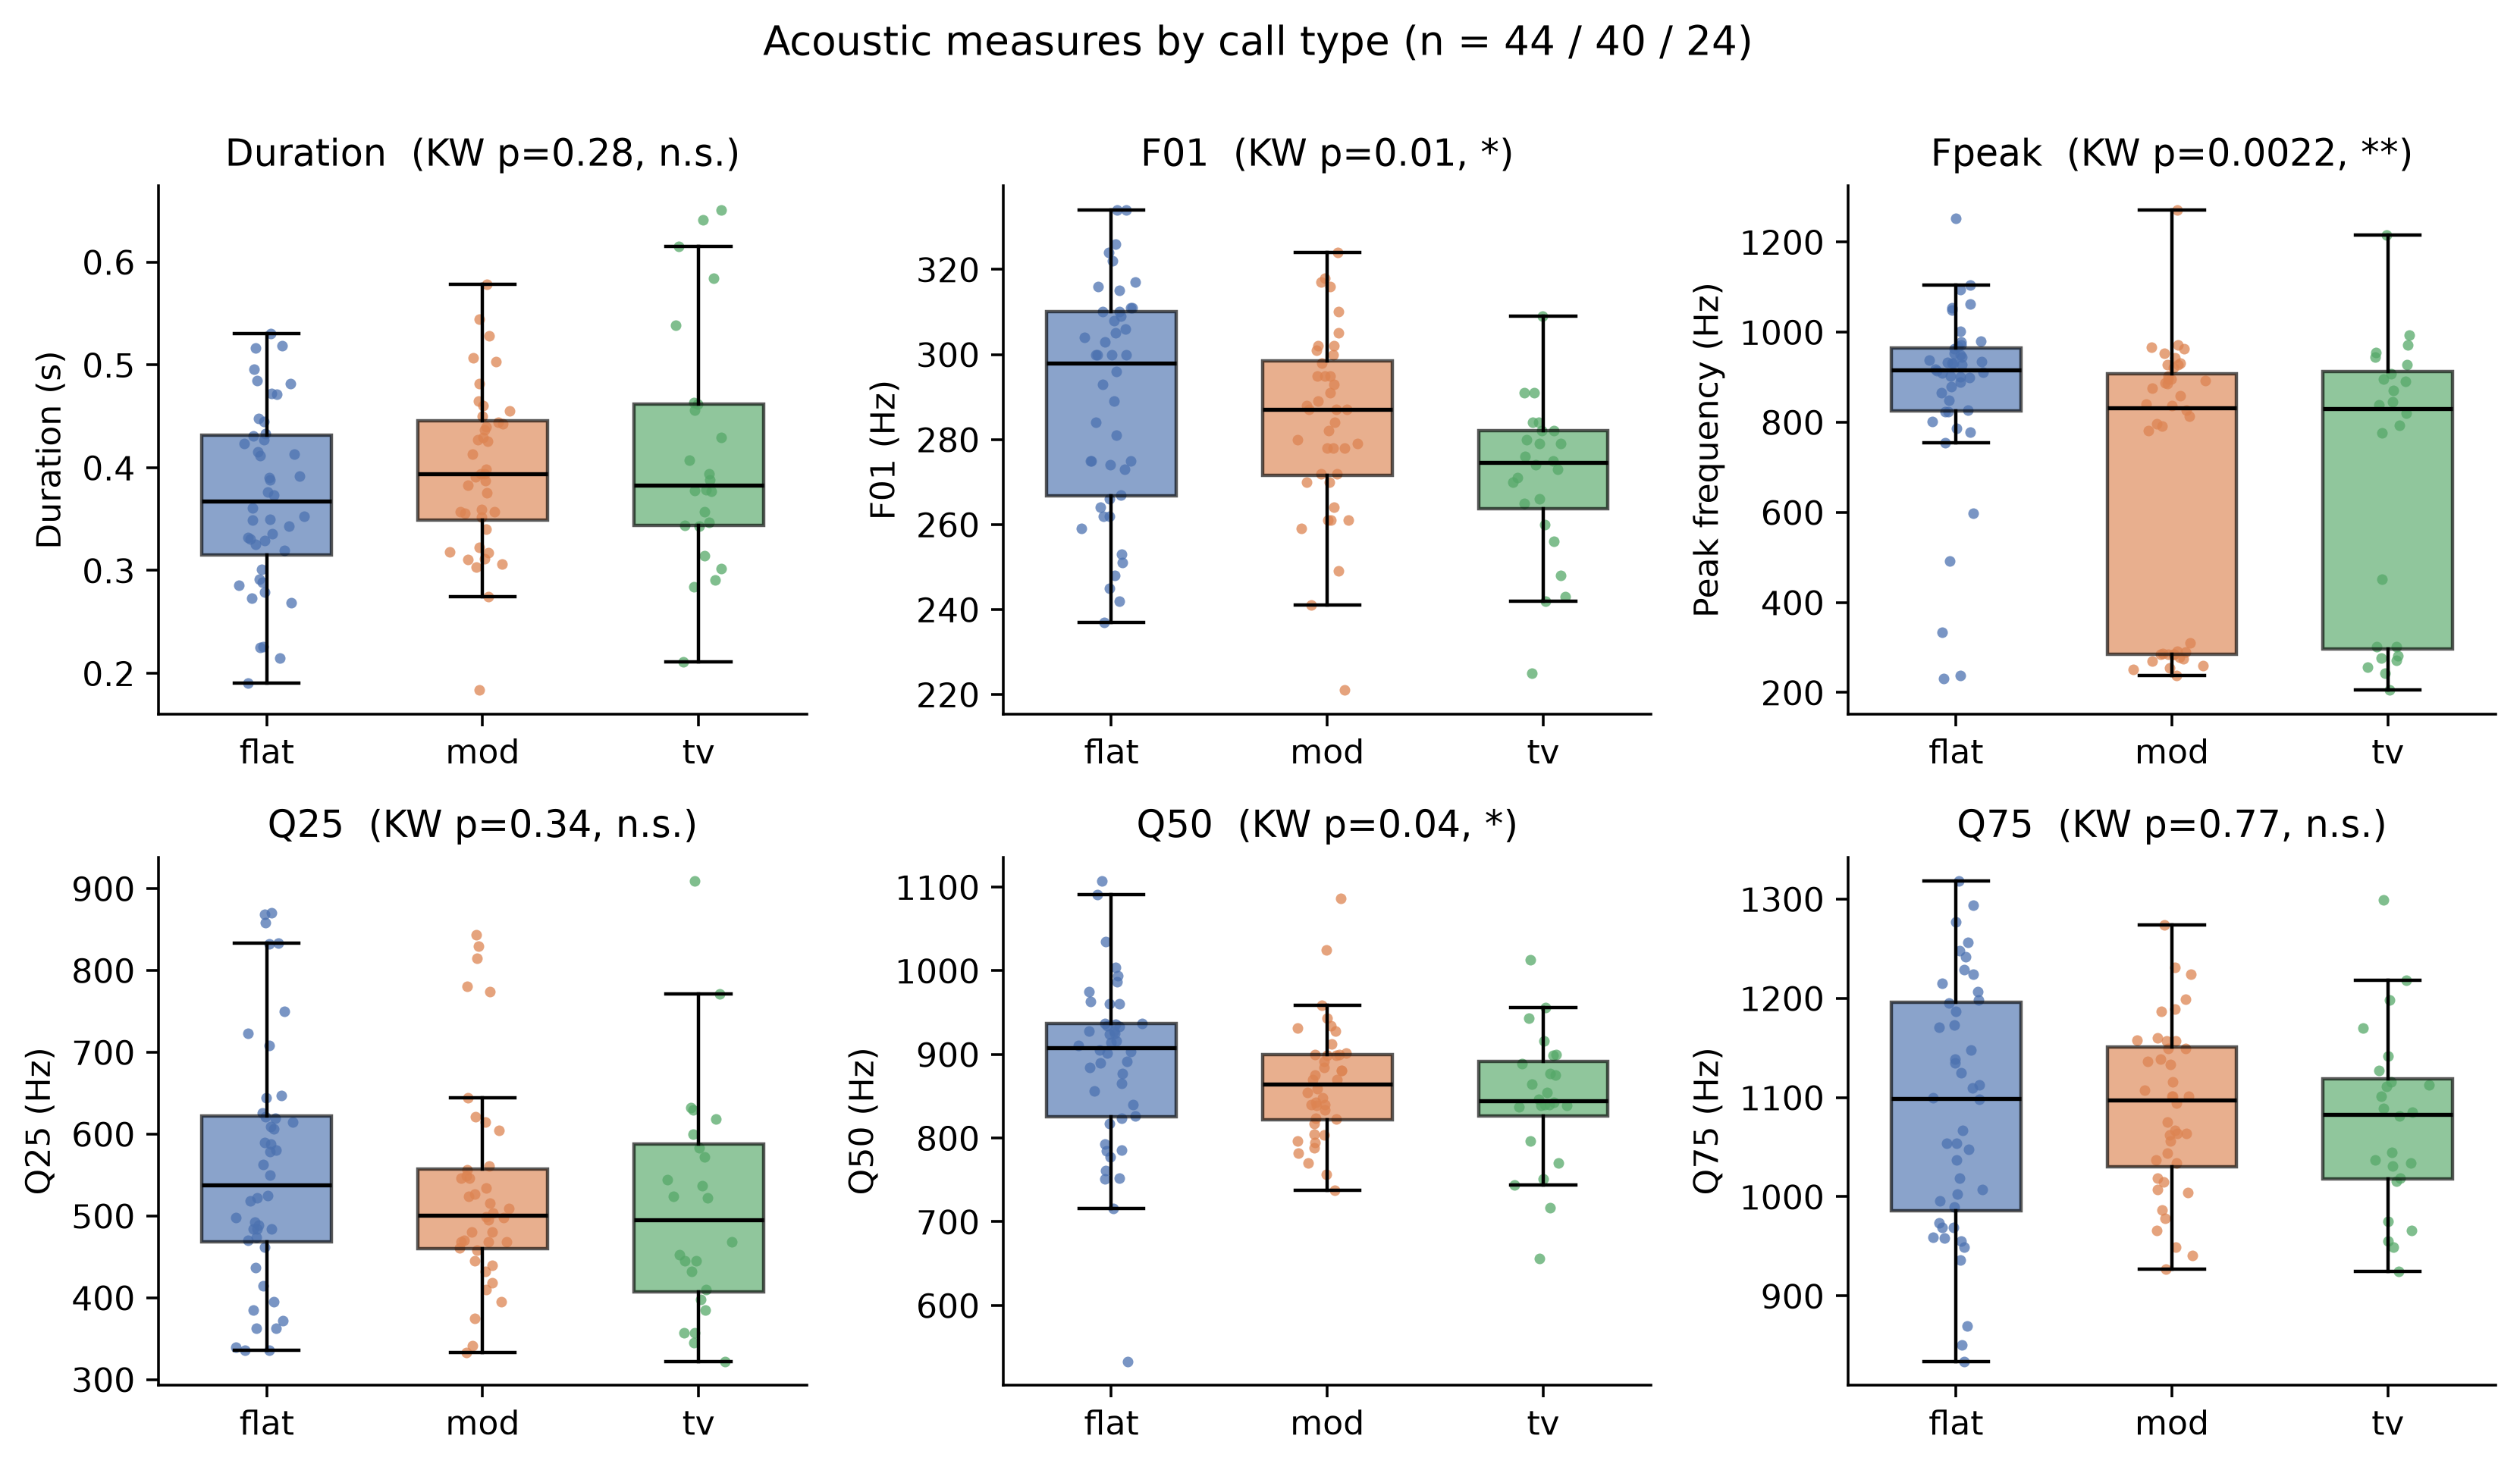
\includegraphics[width=\textwidth]{figures/fig01_boxplots.png}
\caption{Distributions of the six complete acoustic measures by call type. Points are
individual calls, boxes the interquartile range, and the title of each panel gives the
Kruskal--Wallis $p$ value ($^{***}p<0.001$, $^{**}p<0.01$, $^{*}p<0.05$, n.s.\ not
significant).}
\label{fig:box}
\end{figure}

\begin{figure}[!ht]
\centering
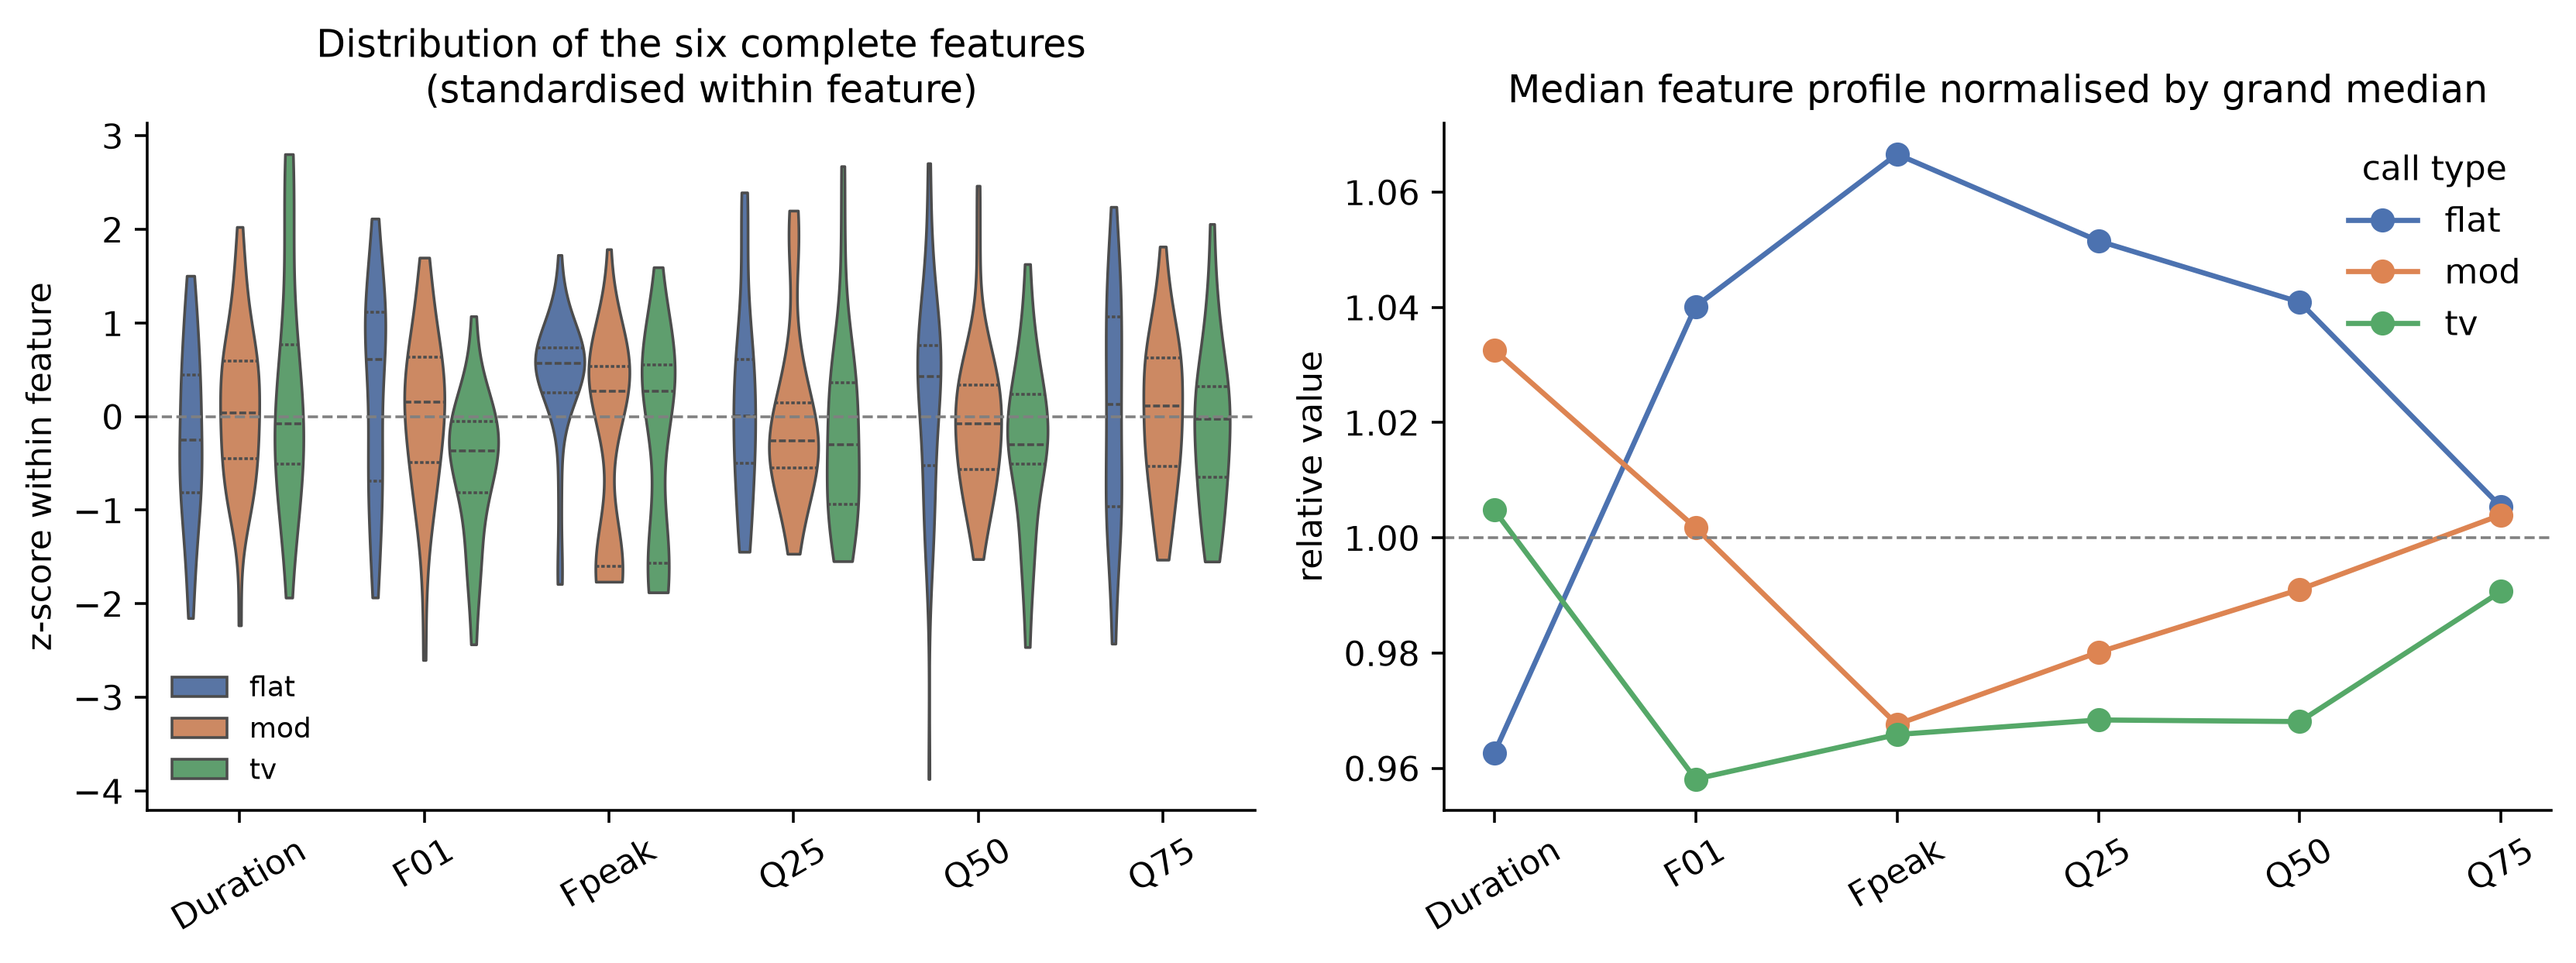
\includegraphics[width=\textwidth]{figures/fig02_violin_profile.png}
\caption{Left: violin plots of the six measures, each standardised within its own feature
so that all six can share one axis, with quartiles marked. Right: median feature profile
of each call type normalised by the grand median, which shows that the three types differ
mainly in the peak-to-median region rather than in overall level.}
\label{fig:violin}
\end{figure}

\subsection{Normality and non-parametric testing}

Shapiro--Wilk tests reject normality in $6$ of the $18$ group-by-measure cells at the
$5\%$ level, mostly in peak frequency and in the lower quartile. With groups of $24$ to
$44$ calls the power of these tests is low, so the rejection is informative only as a
reason to prefer rank-based methods, which the problem requires in any case. We
therefore use the Kruskal--Wallis test\cite{kruskal} as the omnibus test and Dunn's
procedure\cite{dunn} with Benjamini--Hochberg correction\cite{bh} for the three pairwise contrasts, and we report
Mann--Whitney $U$ with the rank-biserial correlation as a sensitivity check rather than
as a second, independent family of tests.

\begin{table}[!ht]
\centering
\caption{Descriptive statistics (median with interquartile range in parentheses) and
Kruskal--Wallis tests of the six complete acoustic measures. $\varepsilon^2$ is the
epsilon-squared effect size.}
\label{tab:desc}
\footnotesize
\begin{tabular}{lcccccc}
\toprule
Measure & flat & mod & tv & $H$ & $p$ & $\varepsilon^2$\\
\midrule
Duration & 0.4 (0.1) & 0.4 (0.1) & 0.4 (0.1) & 2.52 & 0.2832 & 0.005\\
F01 & 298.0 (43.2) & 287.0 (27.0) & 274.5 (18.2) & 9.14 & 0.0103 & 0.068\\
Fpeak & 916.0 (138.8) & 831.0 (621.8) & 829.5 (616.8) & 12.28 & 0.0022 & 0.098\\
$Q_{25}$ & 537.5 (154.2) & 501.0 (97.0) & 495.0 (180.2) & 2.16 & 0.3400 & 0.002\\
$Q_{50}$ & 908.0 (111.5) & 864.5 (78.5) & 844.5 (64.8) & 6.42 & 0.0402 & 0.042\\
$Q_{75}$ & 1099.0 (209.8) & 1097.5 (120.8) & 1083.0 (100.5) & 0.52 & 0.7712 & 0.000\\
\bottomrule
\end{tabular}
\end{table}

\begin{table}[!ht]
\centering
\caption{Dunn post-hoc tests with Benjamini--Hochberg correction ($p$ values) and the
rank-biserial effect size of the flat--tv contrast from the Mann--Whitney
sensitivity check.}
\label{tab:dunn}
\footnotesize
\begin{tabular}{lcccc}
\toprule
Measure & flat--mod & flat--tv & mod--tv & $r_{rb}$ (flat--tv)\\
\midrule
Duration & 0.3210 & 0.3210 & 0.9786 & 0.18\\
F01 & 0.3490 & 0.0079 & 0.0459 & 0.40\\
Fpeak & 0.0042 & 0.0129 & 0.9048 & 0.38\\
Q25 & 0.5094 & 0.4762 & 0.5639 & 0.19\\
Q50 & 0.0855 & 0.0631 & 0.5112 & 0.33\\
Q75 & 0.9829 & 0.7750 & 0.7750 & 0.09\\
\bottomrule
\end{tabular}
\end{table}


Three measures differ significantly across call types
(Table~\ref{tab:desc}): peak frequency ($H=12.28$, $p=0.0022$, $\varepsilon^2=0.098$),
the first fundamental ($H=9.14$, $p=0.010$, $\varepsilon^2=0.068$) and the median
frequency ($H=6.43$, $p=0.040$, $\varepsilon^2=0.042$). Duration, the lower quartile and
the upper quartile show no detectable difference. The effect sizes are small; even the
strongest measure explains under $10\%$ of the rank variance. Dunn's comparisons locate
the peak-frequency difference entirely between flat calls and the two modulated forms
($p=0.0042$ and $p=0.013$, both corrected), while modulated and two-voice calls are
indistinguishable ($p=0.90$). For the first fundamental the contrast is between flat and
two-voice calls ($p=0.0079$). The Mann--Whitney sensitivity check agrees on both
peak-frequency contrasts ($p=0.0013$ and $p=0.011$) and on the flat--two-voice contrast
in the first fundamental ($p=0.0073$), with rank-biserial correlations of absolute size
$0.38$--$0.41$ for these contrasts.

\subsection{Classification and the leakage audit}

Figure~\ref{fig:clf} and Table~\ref{tab:clf} compare three feature sets under identical
five-fold stratified cross-validation. With the six raw measures a random forest\cite{breiman} reaches
$0.481$ accuracy, barely above the $0.407$ majority-class rate, and linear discriminant
analysis and a radial-basis SVM do no better ($0.435$ and $0.472$). The three call types
are therefore not separable by their gross spectral summary statistics.

The three engineered measures change this materially. Spectral bandwidth $Q_{75}-Q_{25}$
expresses how spread out the energy is, while the peak-to-fundamental ratio
$F_{\mathrm{peak}}/F_{01}$ and the median-to-fundamental ratio $Q_{50}/F_{01}$ express
where the energy sits relative to the fundamental, which is the dimension along which a
modulated or two-voice call should differ from a flat one. A random forest on these three
measures reaches $0.639$ accuracy, a gain of $0.158$ over the raw set, with per-class F1
scores of $0.723$ (flat), $0.667$ (modulated) and $0.462$ (two-voice). Out-of-fold
permutation importance is not even: the peak-to-fundamental ratio dominates ($0.205$
decrease in held-out accuracy), the median-to-fundamental ratio follows ($0.131$), and
bandwidth contributes least ($0.053$). In-training Gini importance, by contrast, spreads
almost evenly ($0.358$, $0.344$, $0.299$), showing how correlated predictors share
in-training importance.

Reintroducing the structural flags lifts accuracy to $0.944$, and the linear methods are
affected far less ($0.630$ and $0.935$ for LDA and SVM respectively). The interpretation
is direct: almost all of the practically achievable accuracy on this table comes from
knowing whether a second fundamental exists, which is precisely the label definition. The
$0.639$ figure is the honest estimate of what acoustic shape alone can deliver, and it is
the number we carry forward.

\begin{figure}[!ht]
\centering
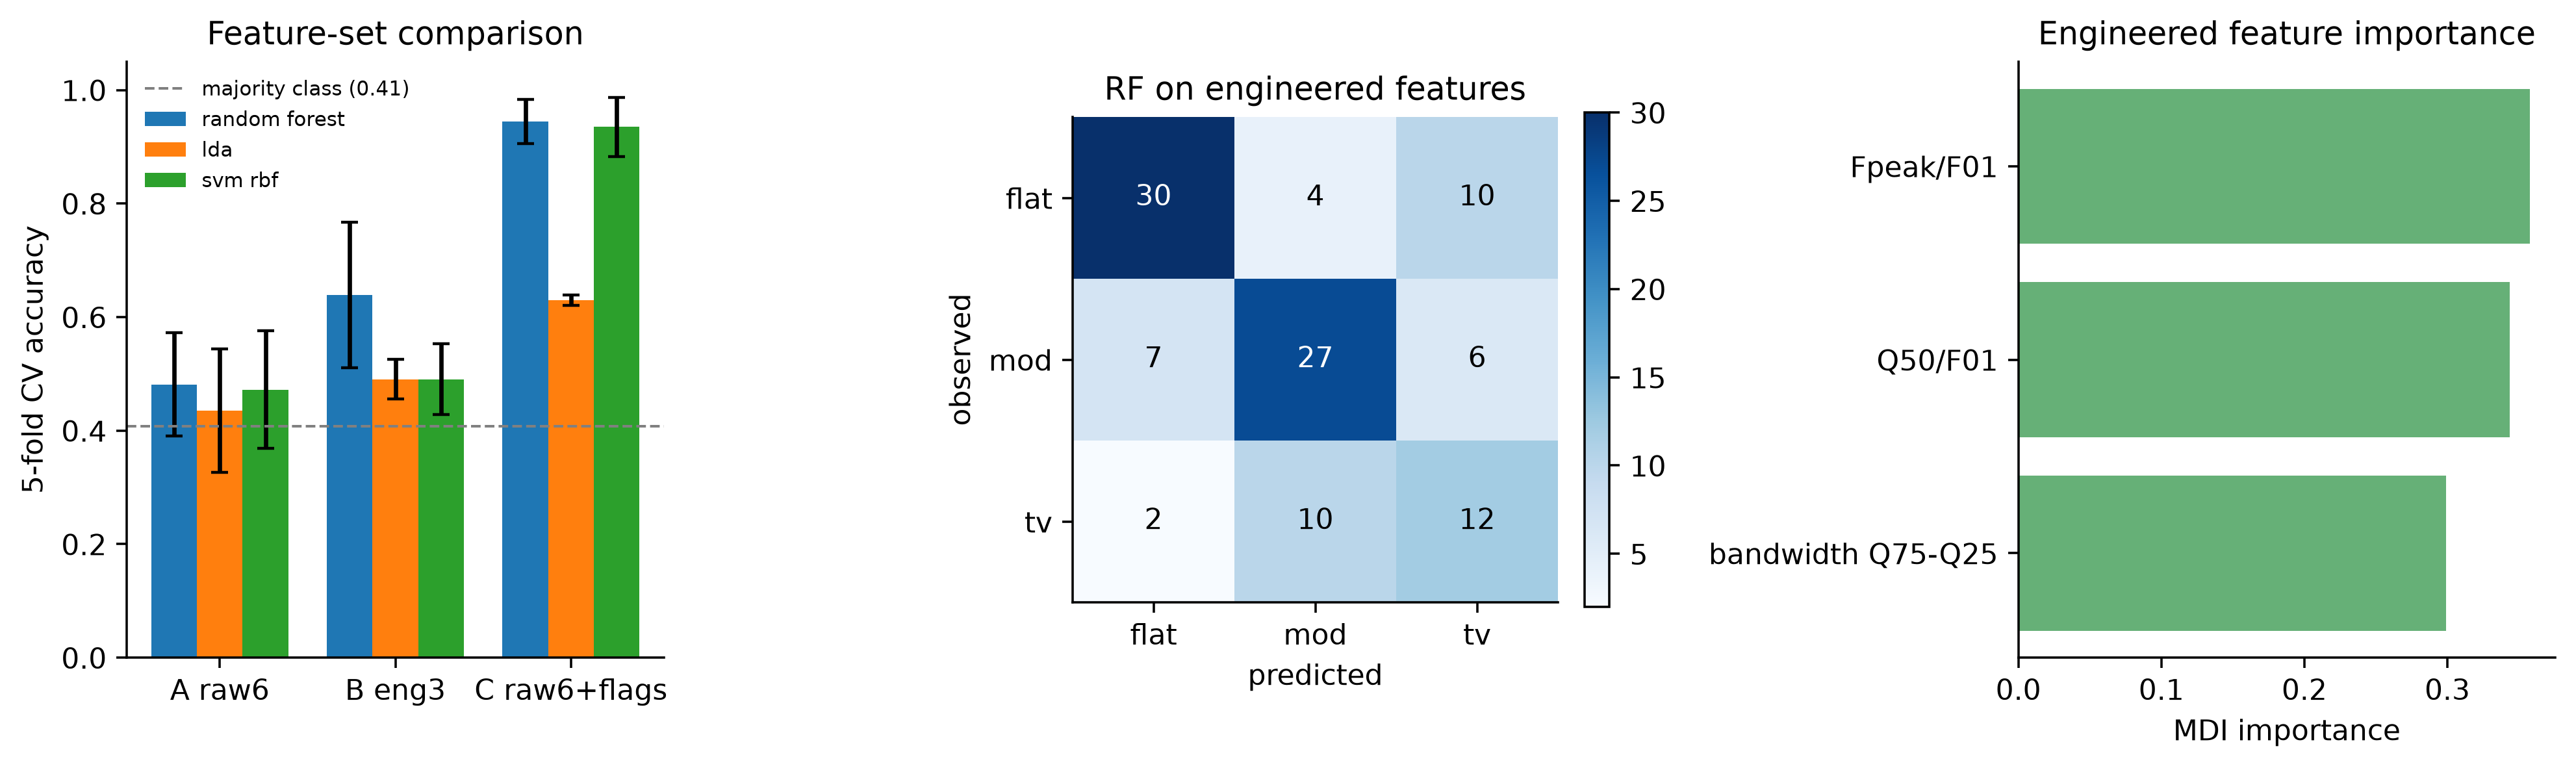
\includegraphics[width=\textwidth]{figures/fig03_classifier.png}
\caption{Left: cross-validated accuracy of three classifiers on three feature sets; the
dashed line is the majority-class rate. Middle: confusion matrix of the random forest on
the engineered measures. Right: importance of the three engineered measures.}
\label{fig:clf}
\end{figure}

\begin{table}[!ht]
\centering
\setlength{\tabcolsep}{4pt}
\caption{Three-class classification of call type (5-fold stratified cross-validation,
$n=108$; majority-class accuracy 0.407). Feature set C is reported only as a leakage
audit and is never used as a substantive classifier. Per-class F1 for the best model
(set B, random forest): flat 0.723, mod 0.667, tv 0.462.}
\label{tab:clf}
\scriptsize
\begin{tabular}{lcccc}
\toprule
Feature set & RF accuracy & LDA accuracy & SVM accuracy & RF macro-F1\\
\midrule
A: six raw measures & 0.481 & 0.435 & 0.472 & 0.469\\
B: three engineered measures & 0.639 & 0.491 & 0.491 & 0.617\\
C: A $+$ structural flags (leakage audit) & 0.944 & 0.630 & 0.935 & 0.952\\
\bottomrule
\end{tabular}
\end{table}


\subsection{Which measures carry forward}

The analysis leaves a clear ranking. Peak frequency and the first fundamental carry the
only defensible between-type effects, and out-of-fold permutation importance confirms the
first fundamental as the most informative raw measure ($0.116$), with peak frequency a
distant second ($0.020$) and the quartiles contributing nothing. The ratios built on
these two quantities are what the classifier actually uses.
For Questions 2 and 3 we therefore retain the spectral-shape quantities (peak and median
frequency relative to the fundamental, and bandwidth) as the interpretable core, and we
treat the presence of a second fundamental and of pulse structure as categorical
descriptors of the vocal mechanism rather than as measurements.

%=====================================================================
\section{Question 2: propagation degradation and communication range}\label{sec:q2}

\subsection{A single fidelity index}

For call type $c$ and metric $m$ let $\bar r_{m}(d)$ be the mean correlation between the
one-metre recording and the recording at distance $d$. The three metrics describe
complementary aspects of the signal: the spectrogram captures time-frequency structure,
the amplitude spectrum captures the spectral envelope, and the amplitude envelope
captures temporal patterning. We define
\begin{equation}
F_c(d)=\sum_{m\in\mathcal{M}} w_m\,\bar r_{m}(d),\qquad \sum_m w_m=1,
\label{eq:fidelity}
\end{equation}
and set $w_m=1/3$. The equal weighting is not assumed but checked: a principal component
analysis of the nine call-by-metric profiles gives loadings of $0.582$, $0.582$ and
$0.569$ on the first component, which explains $96.7\%$ of the variance. The three
metrics are therefore measuring one underlying quantity, and any reasonable weighting
scheme would give nearly the same index.

Figure~\ref{fig:corr} shows the raw decay of the three metrics. All three fall
monotonically after about $16$ m, but they do so at different rates. The envelope
correlation starts lowest, at $0.63$--$0.67$ at $4$ m, because fine temporal structure
is the first thing that a propagating wavefront loses.

\begin{figure}[!ht]
\centering
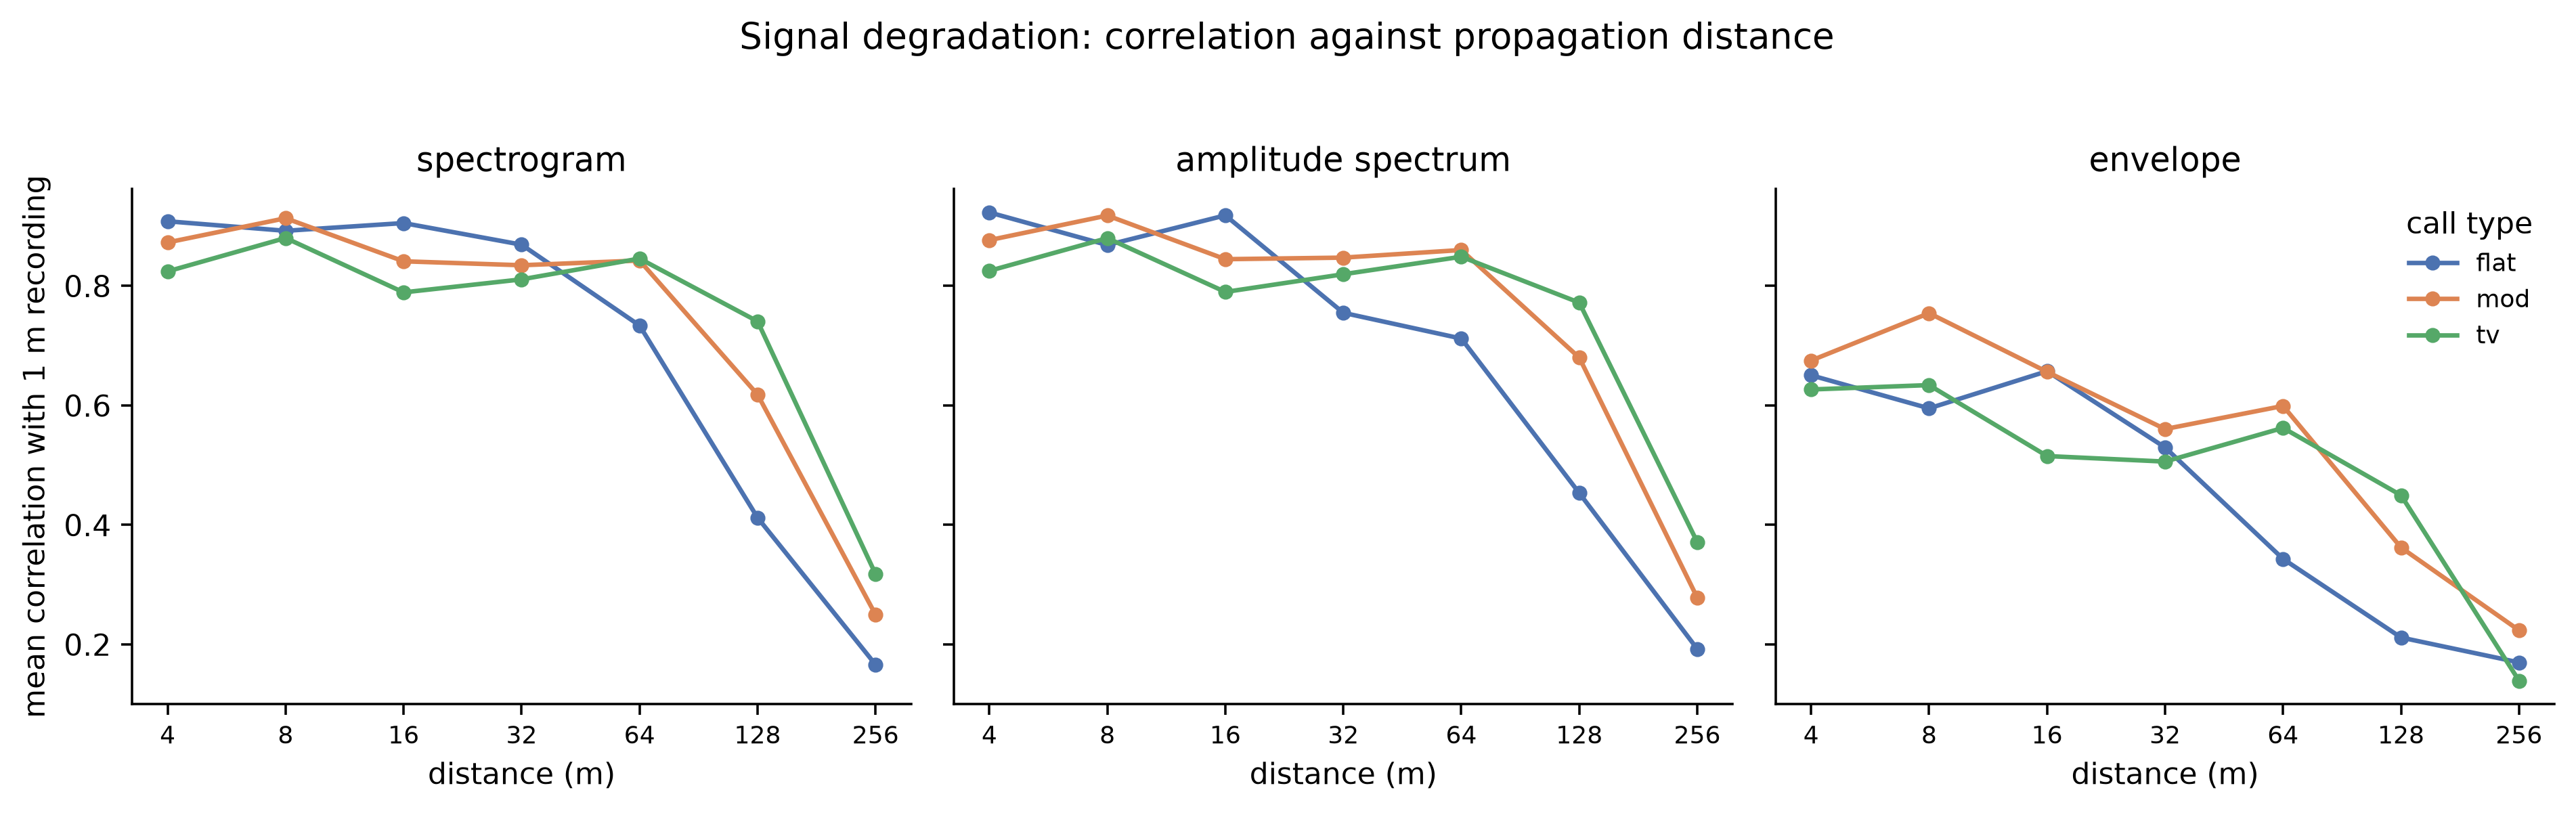
\includegraphics[width=\textwidth]{figures/fig04_correlation_decay.png}
\caption{Mean correlation with the one-metre recording as a function of propagation
distance, for the three metrics and the three call types. Note the logarithmic distance
axis.}
\label{fig:corr}
\end{figure}

The resulting fidelity index falls from $0.827$, $0.808$ and $0.758$ at $4$ m for flat,
modulated and two-voice calls to $0.176$, $0.250$ and $0.276$ at $256$ m. At $64$ m the
values are $0.579$, $0.724$ and $0.728$, and at $128$ m they are $0.388$, $0.575$ and
$0.659$. The ordering is stable across the whole range: the two-voice call retains the
most structure, and the flat call the least.

\subsection{Decay models}

Three candidate forms were fitted by weighted least squares with weights proportional to
the number of usable pairs in each distance cell:
\begin{align}
\text{exponential:}\quad & F(d)=a\,e^{-bd},\\
\text{logistic:}\quad & F(d)=\frac{L}{1+e^{k(d-d_0)}},\\
\text{power:}\quad & F(d)=a\,d^{-b}.
\end{align}
AIC selects\cite{burnham} the exponential form for flat calls and the logistic form for both modulated
and two-voice calls (Table~\ref{tab:decay}). The difference between the exponential and
logistic fits is small for flat calls (AIC $-46.9$ versus $-43.8$), so the selection is
not decisive there, and we carry that ambiguity into the model-form band below. For the
other two call types the logistic form is clearly preferred, which is biologically
plausible: recognition should remain near a plateau and then collapse over a relatively
narrow distance band, rather than decaying smoothly from the first metre.

\begin{table}[!ht]
\centering
\caption{Candidate decay models for the acoustic fidelity index (weighted least
squares, AIC selection; $^{*}$ marks the selected model). Parameters: exponential
$(a,b)$; logistic $(L,k,d_0)$; power $(a,b)$.}
\label{tab:decay}
\footnotesize
\begin{tabular}{llcc}
\toprule
Call type & Model & Parameters & AIC\\
\midrule
flat & exponential & (0.8634, 0.00625) & -46.89$^{*}$\\
flat & logistic & (1.5, 0.009836, 24.33) & -43.80\\
flat & power & (1.266, 0.2206) & -25.75\\
mod & exponential & (0.8664, 0.003983) & -37.79\\
mod & logistic & (0.9518, 0.0115, 164.6) & -43.04$^{*}$\\
mod & power & (1.141, 0.1548) & -25.43\\
tv & exponential & (0.7965, 0.002876) & -33.08\\
tv & logistic & (0.7615, 0.01893, 226.1) & -42.94$^{*}$\\
tv & power & (0.9616, 0.1075) & -25.84\\
\bottomrule
\end{tabular}
\end{table}


\subsection{Effective range and its uncertainty}

We define three recognition tiers on the fidelity index: potential recognition at
$\theta=0.50$, recognition at $\theta=0.60$ and reliable recognition at
$\theta=0.70$. The effective range is the smallest distance at which the fitted curve
crosses the threshold,
\begin{equation}
d^{*}_{c}(\theta)=\min\{d: F_c(d)=\theta\}.
\label{eq:radius}
\end{equation}

Table~\ref{tab:range} reports the results. At the potential-recognition tier the ranges
are $87$ m (flat), $156$ m (modulated) and $192$ m (two-voice); at the stringent tier
they fall to $34$, $76$ and $98$ m. Two-voice calls therefore carry roughly twice the
range of flat calls at every tier.

\begin{table}[!ht]
\centering
\caption{Effective communication range (m) under the three recognition tiers. Columns
2--4 give point estimates of the selected model; the bracket in column 2 is a 95\%
bootstrap interval (1000 whole-recording row-wise resamples preserving the distance
pairing) and column 5 is the range obtained across the three candidate model forms.}
\label{tab:range}
\footnotesize
\begin{tabular}{lcccc}
\toprule
Call & Potential 0.50 [95\% CI] & Recognition 0.60 & Reliable 0.70 & Model-form\\
\midrule
flat & 87.4 [86.1, 88.8] & 58.2 & 33.6 & [67.5, 94.8]\\
mod & 155.8 [152.0, 159.8] & 118.2 & 75.7 & [138.0, 206.4]\\
tv & 191.8 [189.5, 194.0] & 156.7 & 97.6 & [161.9, 437.8]\\
\bottomrule
\end{tabular}
\end{table}


Two sources of uncertainty are reported separately. The bootstrap interval is obtained by
resampling whole recordings (rows) with replacement---preserving the pairing of the same
call across distances and across metrics---and refitting the selected decay model $1000$
times. The intervals are narrow, roughly $\pm1$ m for flat calls and $\pm2$--$4$ m for
modulated and two-voice calls. That narrowness is itself informative: it says that the
sampling error of the distance-specific means is small, and that the dominant uncertainty
lies elsewhere.

The dominant uncertainty is model form. Refitting the same thresholds under the three
candidate decay shapes gives the bands in the last column of Table~\ref{tab:range}:
$[67,95]$ m for flat calls, $[138,206]$ m for modulated calls and $[162,438]$ m for
two-voice calls. The two-voice band is wide because the power law, which fits worst by
AIC, extrapolates a long tail. We therefore quote ranges as intervals rather than point
values, and we do not claim a precise distance for two-voice calls beyond saying that it
exceeds that of the other two types by a substantial margin.

\subsection{Reachability}

Because the envelope correlation is already low at the closest distance, a threshold can
in principle lie above the observed fidelity at $4$ m, in which case Equation
\eqref{eq:radius} has no solution and the correct report is ``$\le 4$ m, below the
observation limit'' rather than a manufactured number. For the combined index this regime
never arises: the lowest value of $F_c(4)$ across call types is $0.758$, above even the
strictest threshold, so every reported radius is an interior solution and not a grid
endpoint. Per metric the picture is sharper. The envelope correlation at $4$ m is
$0.63$--$0.67$, which lies \emph{below} the $0.70$ reliable-recognition threshold, so for
the envelope metric alone every call type would be reported ``$\le 4$ m''. The two spectral
metrics do not have this problem, with $4$ m correlations of $0.82$--$0.92$. Combining the
three metrics in Equation~\eqref{eq:fidelity} is therefore not a convenience but a
necessity: it is what makes the reliable-recognition threshold reachable in the first
place, and we record this rule explicitly because it is easy to violate when thresholds
are tuned upward.

\begin{figure}[!ht]
\centering
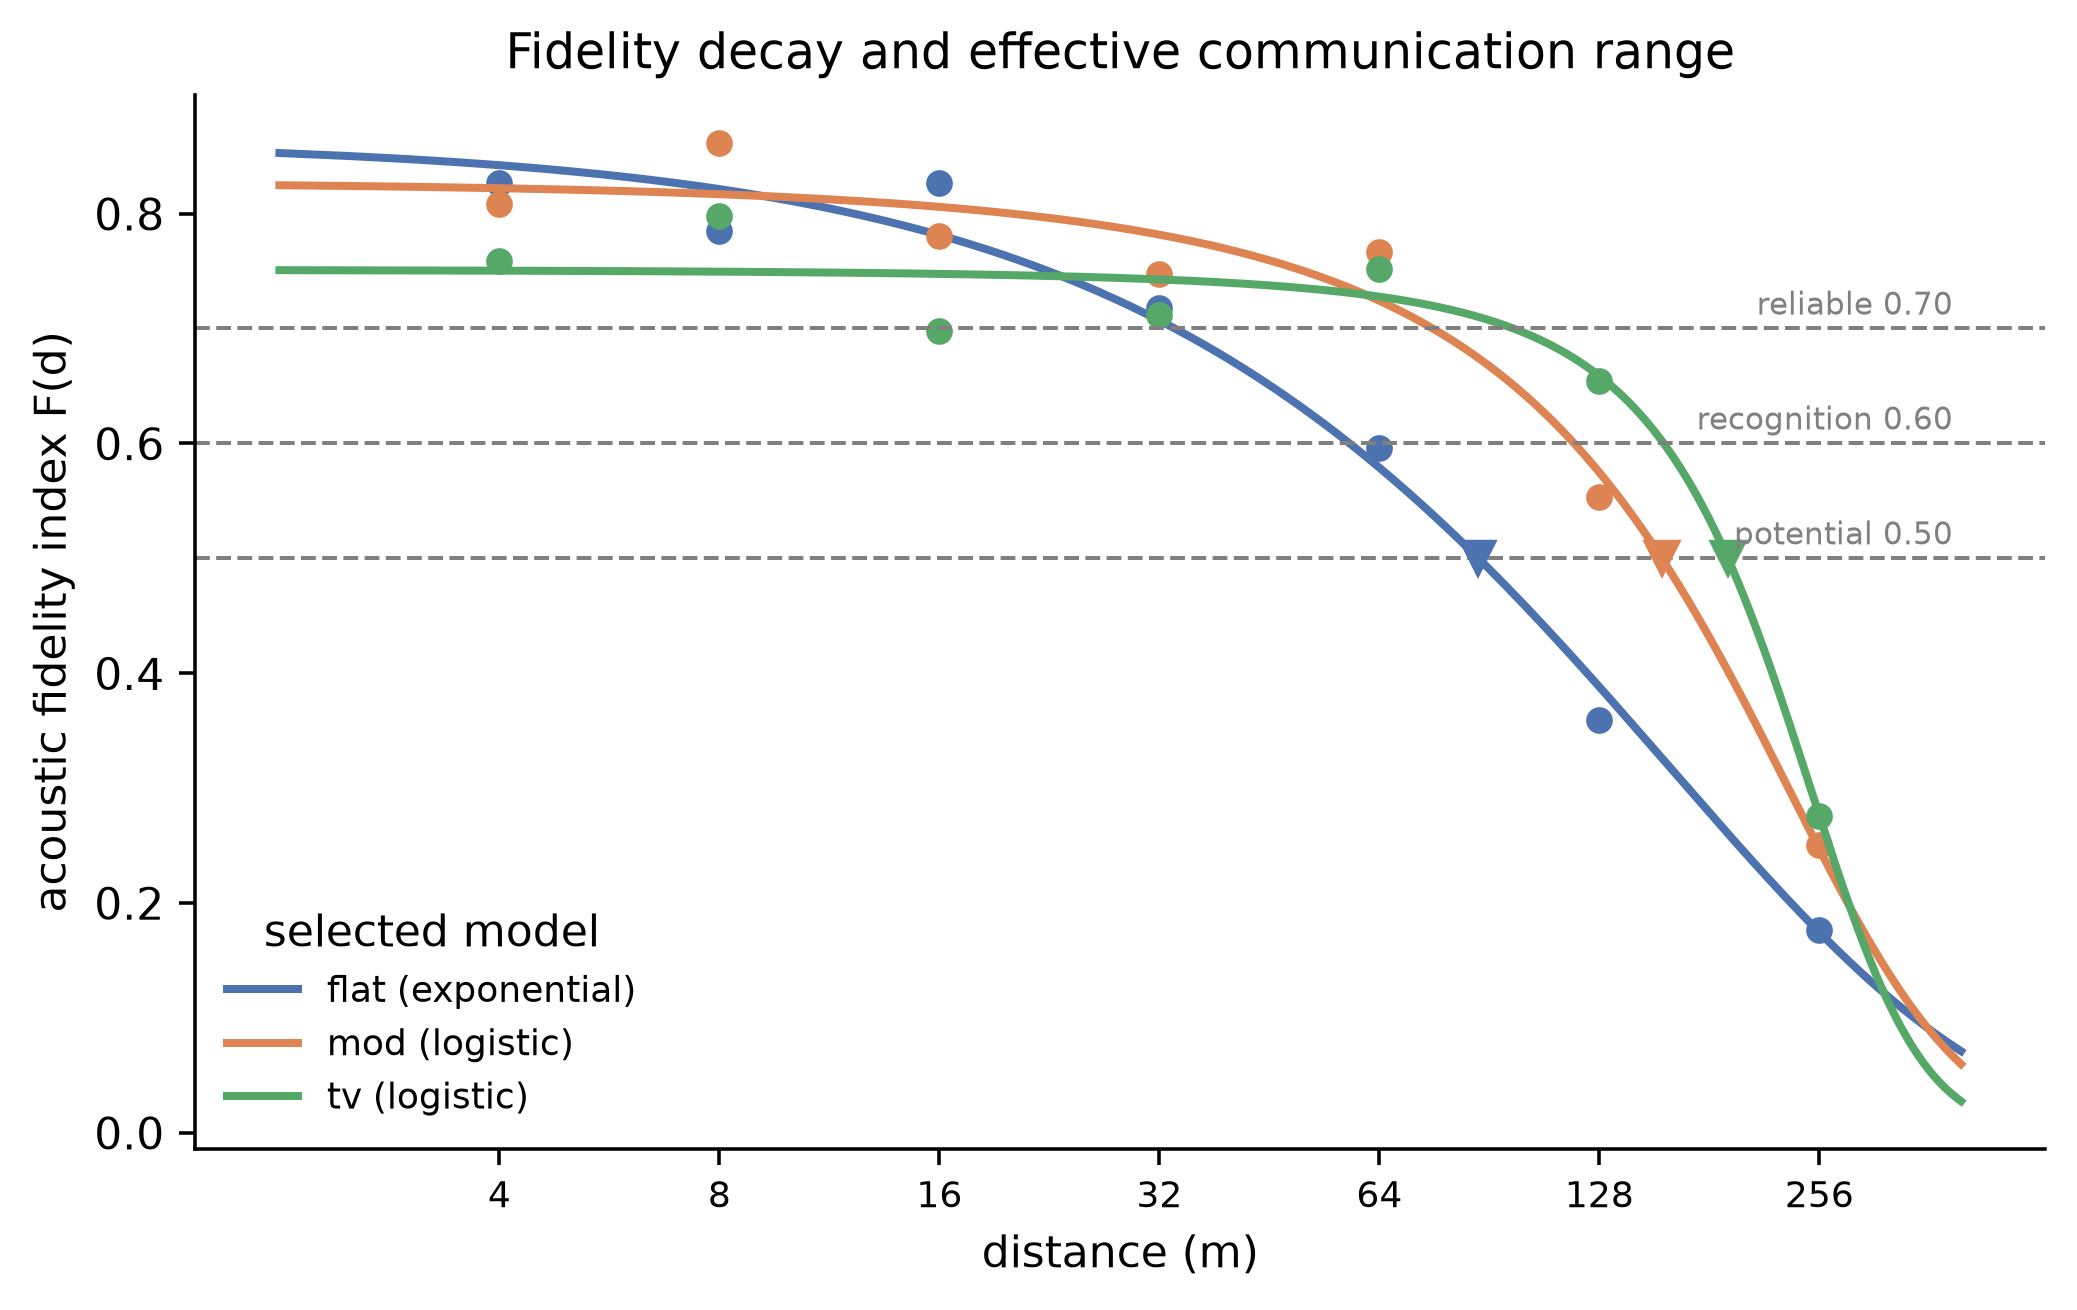
\includegraphics[width=0.78\textwidth]{figures/fig05_fidelity_range.png}
\caption{Fidelity index with the selected decay curve for each call type. Horizontal
dashed lines are the three recognition tiers; inverted triangles mark the
potential-recognition range.}
\label{fig:range}
\end{figure}

\begin{figure}[!ht]
\centering
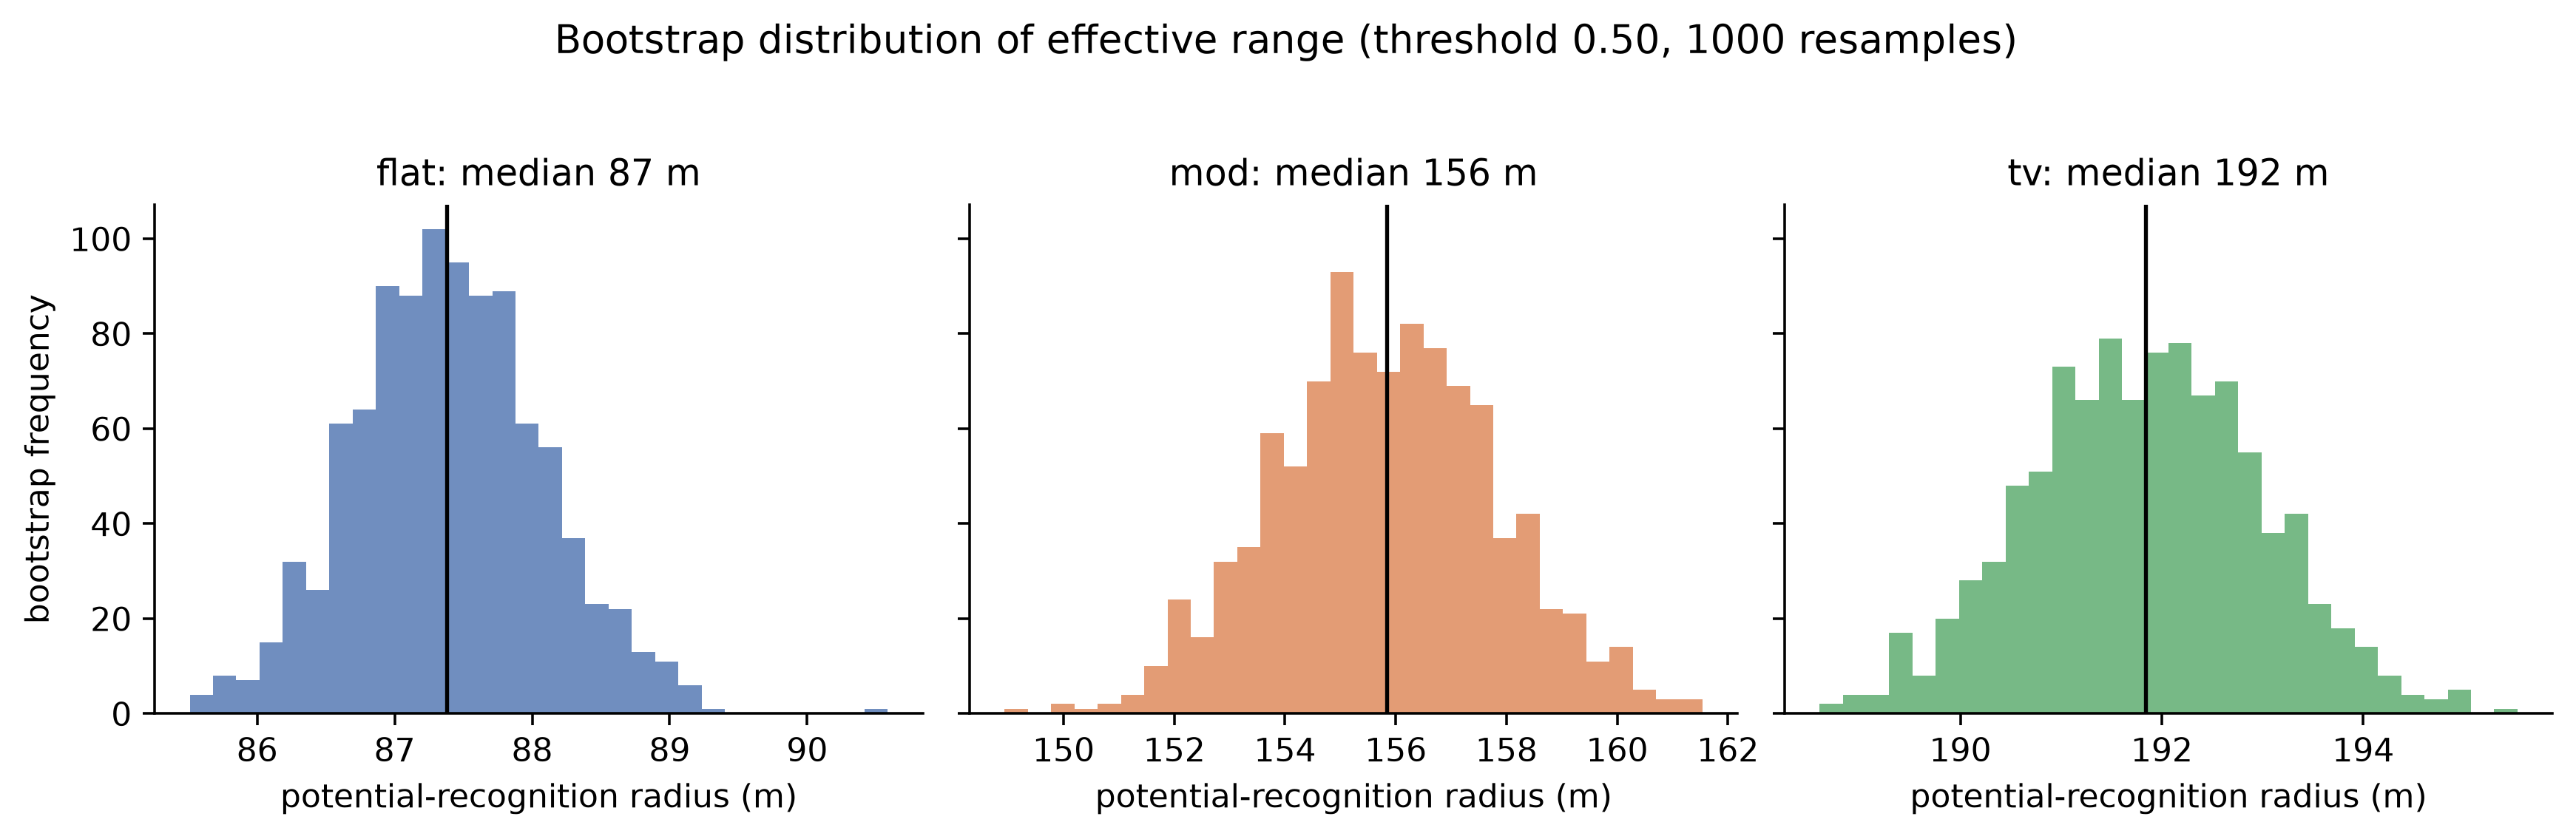
\includegraphics[width=\textwidth]{figures/fig06_bootstrap_range.png}
\caption{Bootstrap distributions of the potential-recognition range, $1000$ resamples
per call type. The distributions are narrow because the dominant uncertainty is model
form rather than sampling error.}
\label{fig:boot}
\end{figure}

\subsection{Which call travels best}

The ranking is unambiguous and consistent across every summary: fidelity at $64$, $128$
and $256$ m, all three thresholds, and all three model forms. Two-voice calls rank first,
modulated calls second and flat calls third. At $256$ m the fidelity indices are $0.276$,
$0.250$ and $0.176$. The mechanism is consistent with the acoustic structure described in
Question~1: a two-voice call carries energy at two fundamentals, so the receiver has two
partially redundant representations of the same signal. The advantage is carried mainly
by the amplitude-spectrum and spectrogram correlations, which at $256$ m are $0.365$ and
$0.311$ for two-voice calls against $0.169$ and $0.138$ for flat calls. The envelope
correlation behaves differently: it decays fastest and is almost identical across call
types at long range ($0.141$ for two-voice against $0.163$ for flat calls), which is
expected because fine temporal structure is lost before spectral structure.

%=====================================================================
\section{Question 3: behavioural responses to playback}\label{sec:q3}

\subsection{Overall response rates}

Natural calls elicited a response in $90$ of $139$ trials ($64.8\%$), control sounds in
$18$ of $139$ ($12.9\%$). The difference is large and unambiguous
($\chi^2=78.49$, $p=8.0\times10^{-19}$, Cram\'er's $V=0.531$; Fisher exact odds ratio
$12.3$ in favour of natural calls, $p=1.9\times10^{-19}$; risk difference $0.518$). This is
the backbone result of
the question: penguins at sea do respond to conspecific calls, and the response is not a
general reaction to any underwater sound.

\begin{figure}[!ht]
\centering
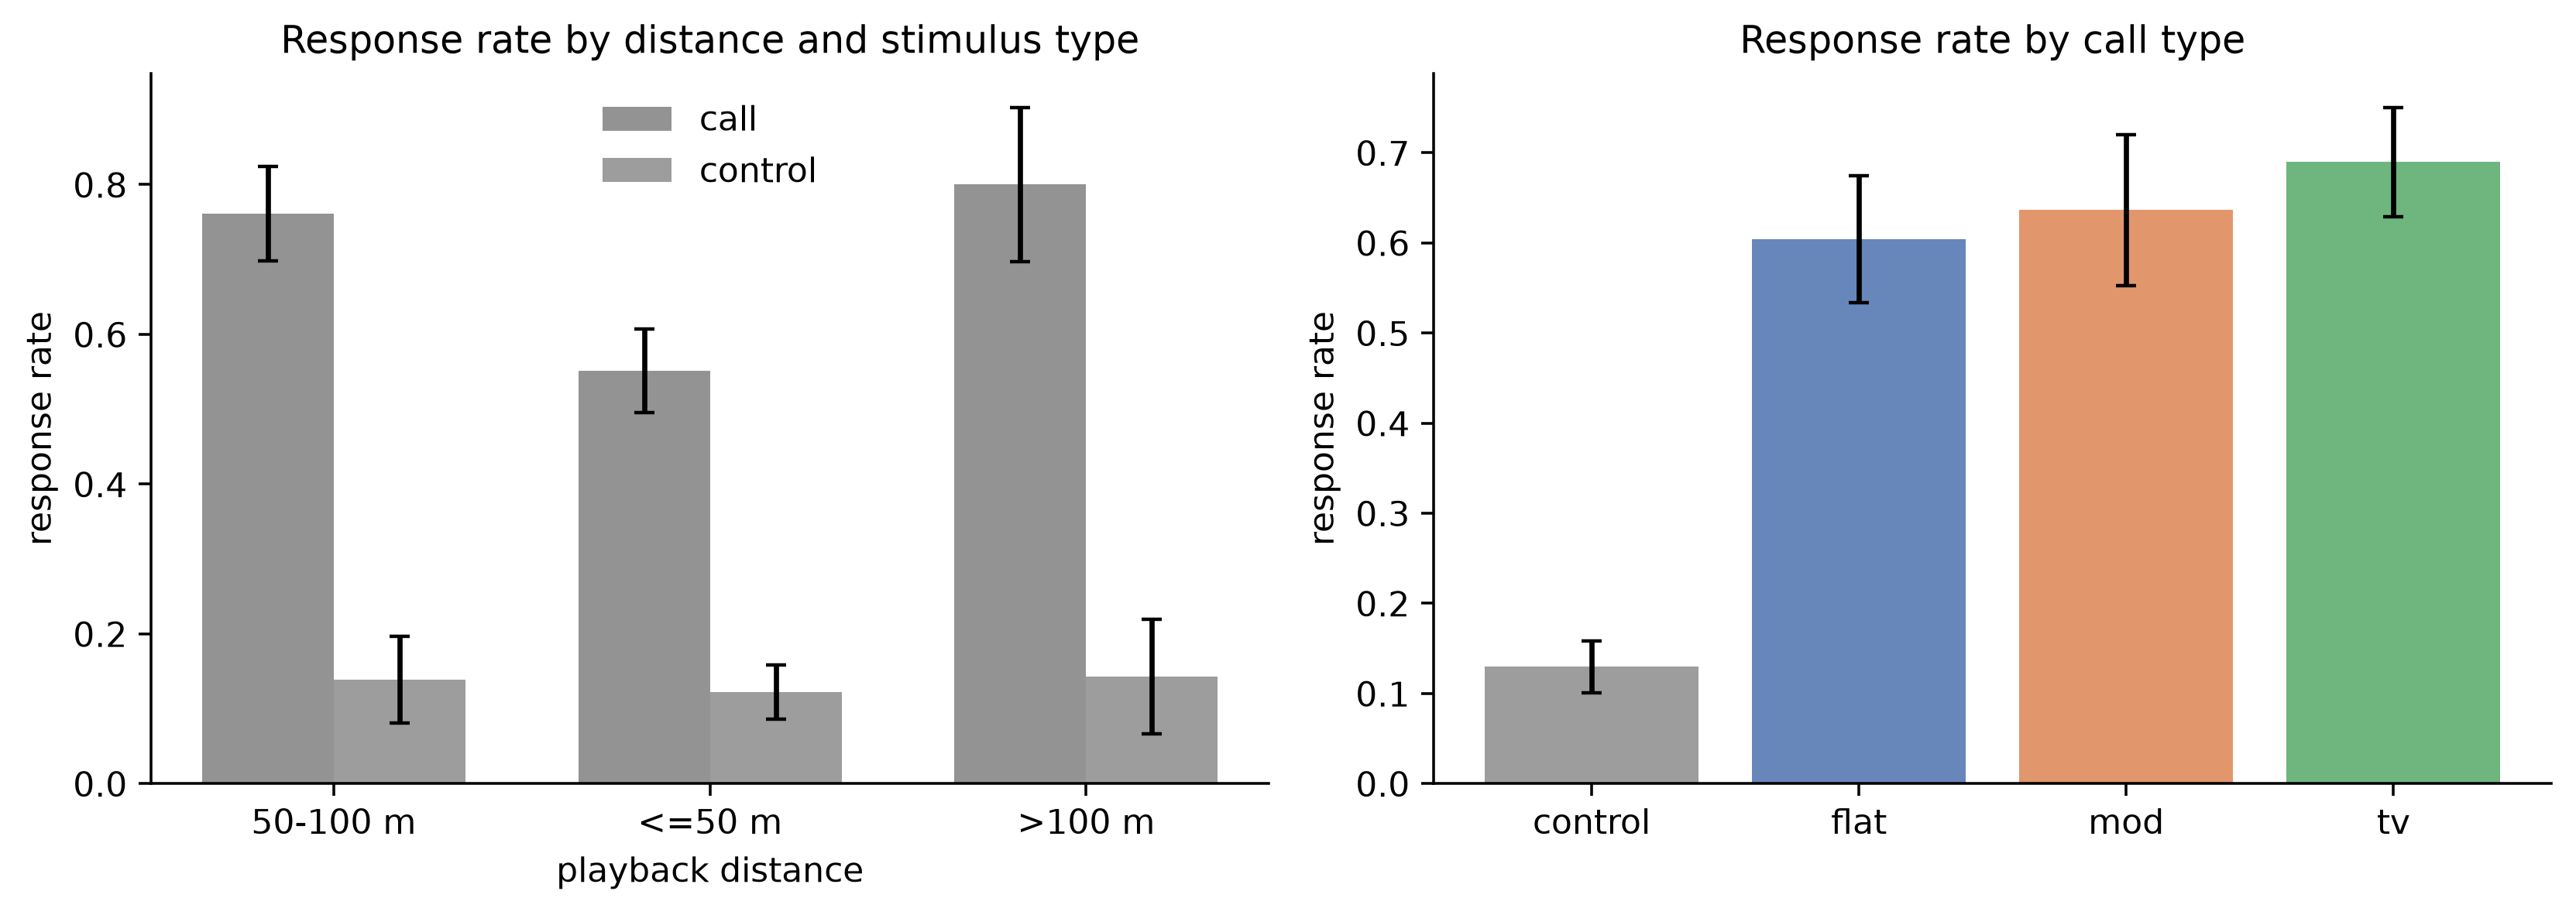
\includegraphics[width=\textwidth]{figures/fig07_response_rate.png}
\caption{Left: response rate by distance class and stimulus type, with binomial standard
errors. Right: response rate by call type, including the control class.}
\label{fig:rate}
\end{figure}

\subsection{Logistic models of the response probability}

Table~\ref{tab:logit} reports two binomial logit models. The pooled model uses all $278$
trials and six parameters, giving about $18$ events per parameter. Holding context and
distance at their reference values, a control stimulus multiplies the odds of a response
by $0.058$ (95\% CI $[0.029,0.115]$). Each tenfold increase in distance multiplies the
odds by $0.21$ ($[0.069,0.642]$), and each additional penguin in the observed group
multiplies them by $0.941$ ($[0.903,0.979]$). The group-size effect is small per
individual but consistent: larger groups respond at a slightly lower rate, which is
compatible with individual vigilance being diluted in a larger aggregation, and it
reappears in every behavioural sub-model. Context does not reach significance in the
pooled model.

\begin{table}[!ht]
\centering
\caption{Binomial logistic models of the probability of any response. Pseudo-$R^2$
of the pooled model is 0.310 (AIC 268.2).}
\label{tab:logit}
\footnotesize
\begin{tabular}{lccc}
\toprule
Term & Odds ratio & 95\% CI & $p$\\
\midrule
\multicolumn{4}{l}{Pooled model (reference: natural call, context: after)}\\
\quad $\log_{10}$ distance & 0.210 & [0.069, 0.642] & 0.0062\\
\quad group size & 0.941 & [0.903, 0.979] & 0.0031\\
\quad stimulus = control & 0.058 & [0.029, 0.115] & 0.0e+00\\
\quad context: commuting & 0.796 & [0.374, 1.695] & 0.5537\\
\quad context: searching & 1.879 & [0.757, 4.662] & 0.1738\\
\midrule
\multicolumn{4}{l}{Call-only model (reference: flat, context: after)}\\
\quad call type = mod & 1.230 & [0.433, 3.489] & 0.6975\\
\quad call type = tv & 1.590 & [0.635, 3.981] & 0.3223\\
\quad $\log_{10}$ distance & 0.268 & [0.056, 1.272] & 0.0975\\
\quad group size & 0.938 & [0.895, 0.983] & 0.0075\\
\bottomrule
\end{tabular}
\end{table}


The call-only model isolates differences among the three natural call types on the $139$
natural trials. Neither modulated nor two-voice calls differ significantly from flat calls
(odds ratios $1.23$ and $1.59$, $p=0.70$ and $p=0.32$). Distance attenuates the response
more weakly within this subset (odds ratio $0.268$ per decade, $p=0.098$), which is
expected because the control trials, which carry much of the distance signal, are
excluded. Searching context raises the odds about ninefold relative to the after-context
baseline ($[1.77,47.29]$, $p=0.008$), though that interval is wide and the estimate rests
on a modest number of trials.

\subsection{The three behaviours separately}

Applying the ten-events-per-covariate budget before fitting, head raising ($68$ events)
and vocalising ($81$ events) support five covariates, while approaching ($23$ events)
supports at most two. The fitted models are consistent with the pooled one: for head
raising, natural calls multiply the odds by $7.23$ ($[3.57,14.61]$), distance by $0.132$
per decade ($[0.045,0.389]$) and group size by $0.938$ per penguin ($[0.895,0.983]$),
with pseudo-$R^2=0.194$. For vocalising the stimulus effect is much larger (odds ratio
$49.6$) and the distance effect is not significant, with pseudo-$R^2=0.381$.

Approaching cannot be analysed this way. All $23$ approach events occurred in natural-call
trials and none in the $139$ control trials, so the stimulus coefficient is separated and
any multivariable fit diverges. We report the single-factor tests instead. The log-rank
test for time to approach nevertheless rejects equality of the two stimulus groups
($p=5.7\times10^{-7}$), and a one-covariate Cox model within the natural-call trials gives
a distance hazard ratio of $0.33$ ($[0.11,0.99]$, $p=0.056$). This is the correct
treatment: the stimulus effect is reported as a qualitative separation rather than as a
numerical odds ratio.

\subsection{How many behaviours at once}

Because the three behaviours are not independent, we also model the number of behaviours
observed in a trial, a count from zero to three. A proportional-odds ordered logit was
fitted first, but a likelihood-ratio test against the unrestricted multinomial alternative
rejects the proportional-odds restriction ($\mathrm{LR}=23.14$, $\mathrm{df}=12$,
$p=0.027$). We therefore report the multinomial model: its AIC ($473.17$) is marginally
higher than that of the restricted model ($472.31$), but the likelihood gain justifies the
extra parameters once the proportionality assumption is rejected. Its implied
distributions are stark: for control stimuli the predicted shares of zero, one, two and
three behaviours are $0.871$, $0.129$, $0.000$ and $0.000$, whereas for natural calls they
are $0.353$, $0.288$, $0.259$ and $0.101$. Natural calls do not merely raise the
probability of some response; in this sample they also change the shape of the response
profile, multi-behaviour responses being observed almost exclusively under natural-call
playbacks. Because the control group contains no approach events, this difference is a
sample observation rather than an estimated causal effect size.

\begin{figure}[!ht]
\centering
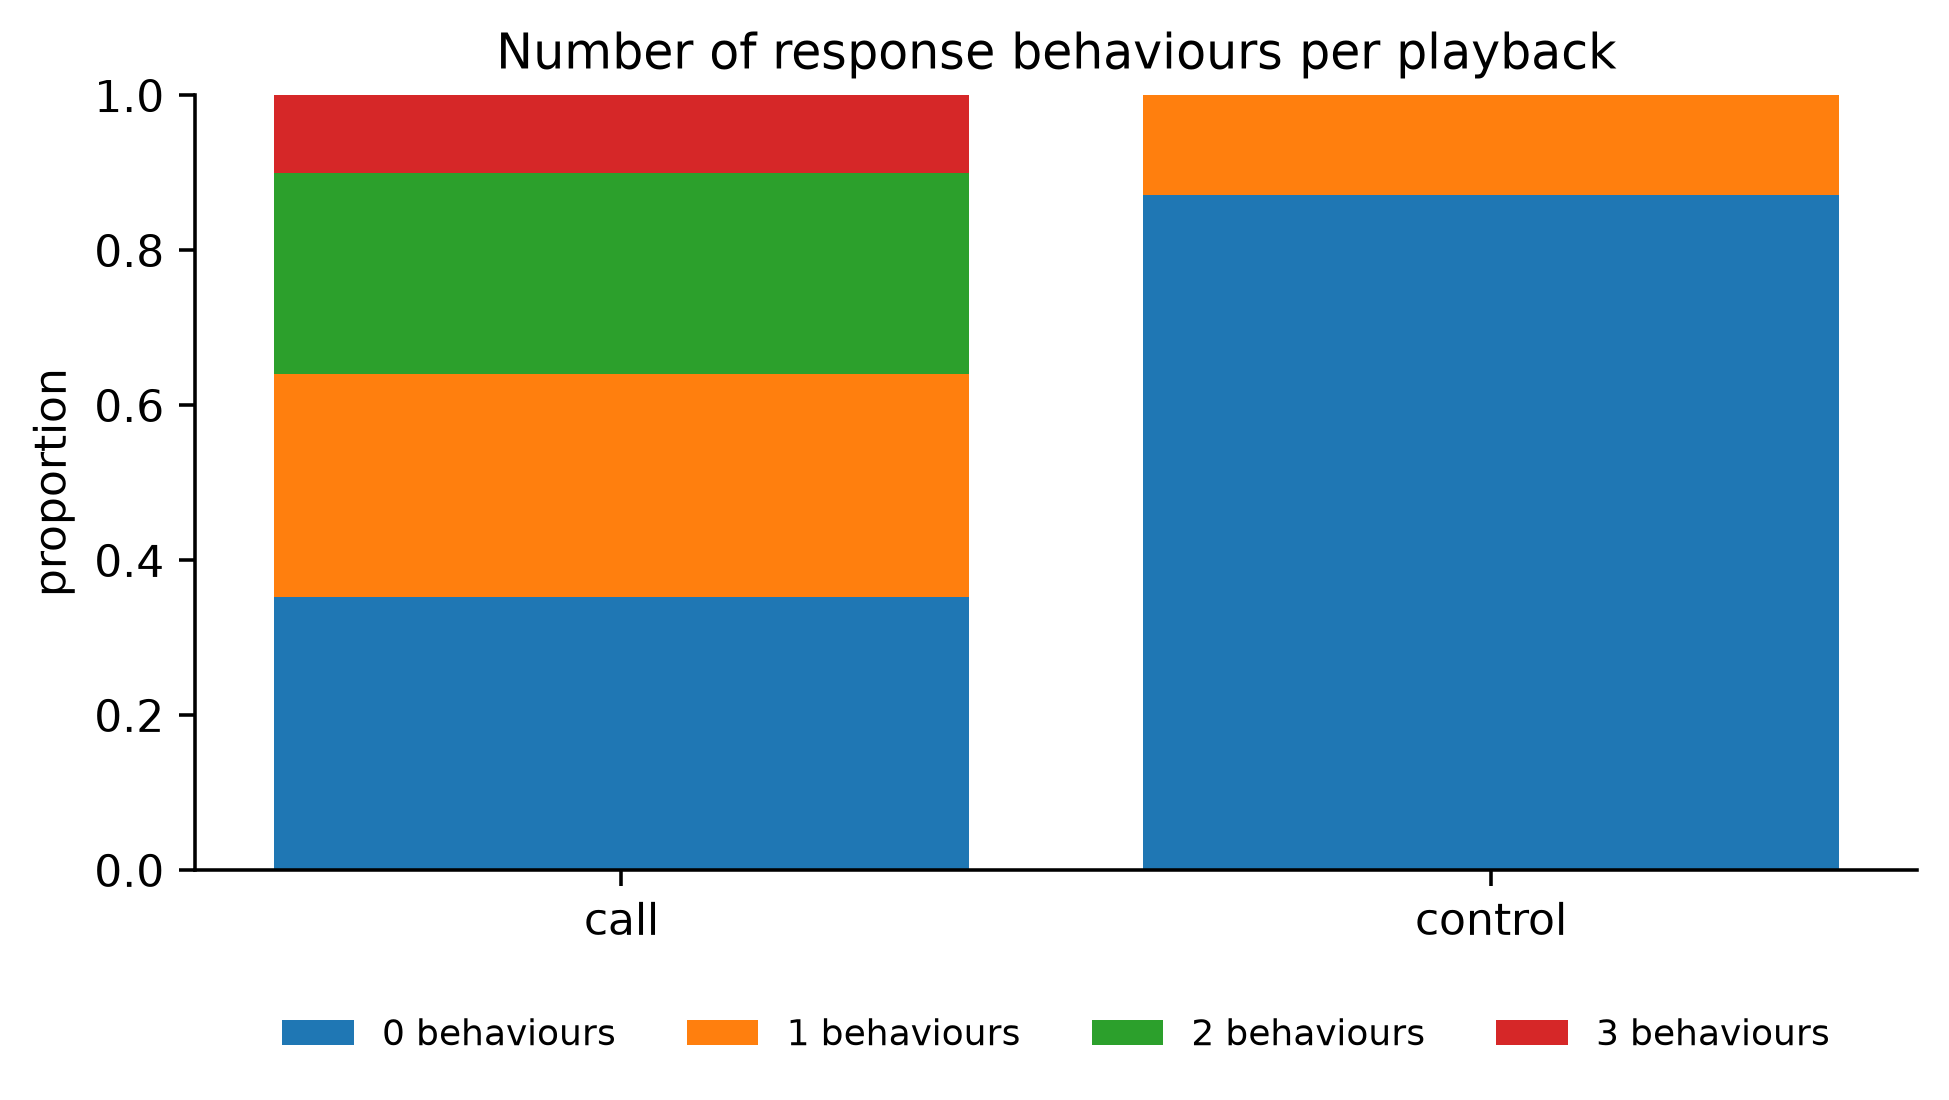
\includegraphics[width=0.62\textwidth]{figures/fig08_behaviour_count.png}
\caption{Distribution of the number of response behaviours per playback trial, separated
by stimulus type.}
\label{fig:nbeh}
\end{figure}

\subsection{Response latency as a censored outcome}

A trial in which no behaviour is recorded is not a trial in which the stimulus was not
perceived, so non-responses are treated as right-censored. The data do not state the
observation window, so non-responses are censored at a surrogate time equal to the longest
observed latency ($10.0$ s head raising, $47.8$ s vocalising, $34.0$ s approaching), an
assumption tested below. Four vocalising and five approaching trials record a latency with
a zero flag; these are kept as censored rather than silently dropped.

Figure~\ref{fig:km} and Table~\ref{tab:surv} give the Kaplan--Meier\cite{km} curves and Cox\cite{cox} models.
The stimulus effect is strong for all three behaviours: hazard ratios of $4.90$
($[2.68,8.98]$) for head raising and $21.66$ ($[8.75,53.61]$) for vocalising, with
C-indices of $0.726$ and $0.756$. Distance attenuates the head-raising hazard
($0.247$ per decade, $[0.124,0.492]$) but not the vocalising hazard, which is compatible
with vocalising being a short-range, within-group signal while head raising is directed at
more distant stimuli. Varying the surrogate censoring time over $0.5\times$--$1.5\times$
leaves the head-raising hazard ratio almost unchanged ($4.4$--$4.9$) but moves the
vocalising ratio between $21.7$ and $26.9$; the effect remains strongly positive throughout.

\begin{figure}[!ht]
\centering
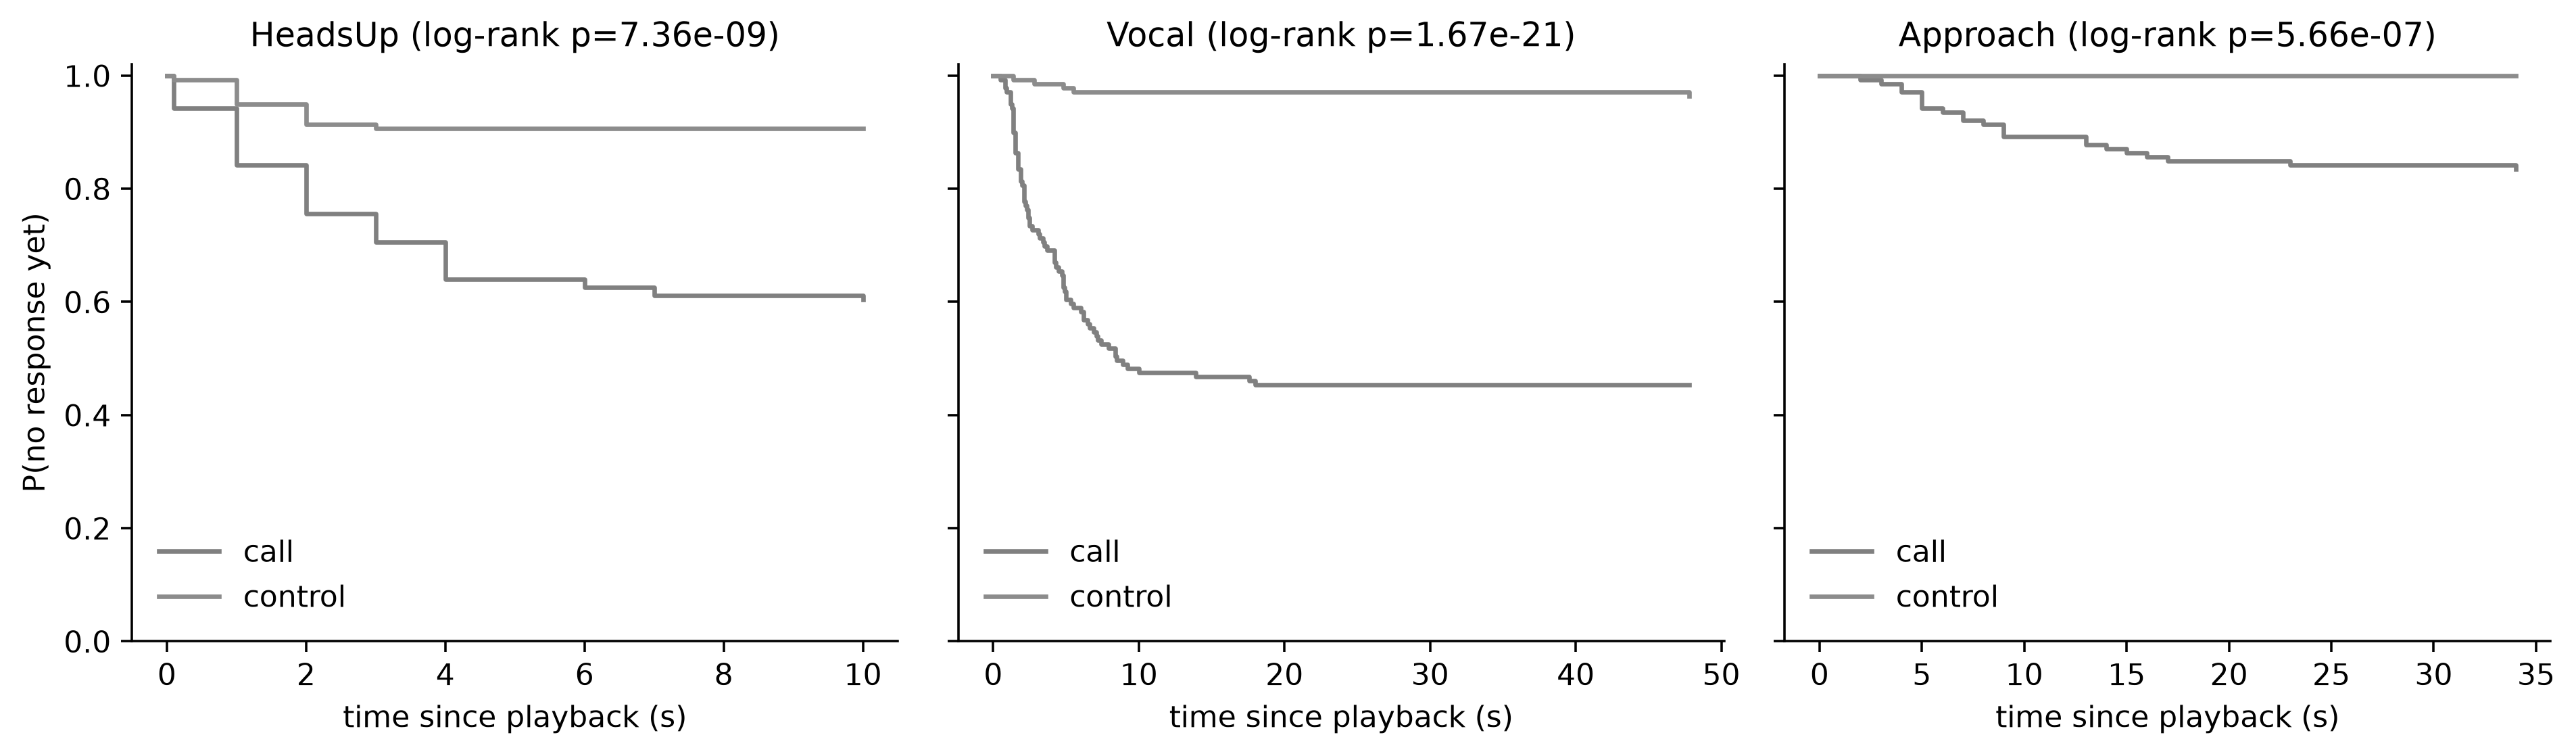
\includegraphics[width=\textwidth]{figures/fig09_km_latency.png}
\caption{Kaplan--Meier curves of the time to each response behaviour, natural calls
against control sounds. Non-responses are right-censored at the observation window.}
\label{fig:km}
\end{figure}

\begin{table}[!ht]
\centering
\setlength{\tabcolsep}{4pt}
\caption{Latency models with right-censoring. Each Cox model uses at most two
covariates, so the events-per-variable ratio stays above 10. The last column reports
scaled Schoenfeld residual $p$ values. $^{a}$All 23 approach events occurred in
natural-call trials (none in 139 control trials), so the stimulus coefficient is not
estimable; the log-rank test remains valid.}
\label{tab:surv}
\scriptsize
\begin{tabular}{lcccccc}
\toprule
Behaviour & Events & Log-rank $p$ & HR (call) & HR ($\log_{10}d$) & C-index & PH test $p$\\
\midrule
HeadsUp & 68 & 7.4e-9 & 4.90 [2.68, 8.98] & 0.25 [0.12, 0.49] & 0.726 & call=0.065, $\log_{10}d$=0.478\\
Vocal & 81 & 1.7e-21 & 21.66 [8.75, 53.61] & 1.18 [0.49, 2.80] & 0.756 & call=0.774, $\log_{10}d$=0.006\\
Approach & 23 & 5.7e-7 & n.e.$^{a}$ & 0.33 [0.11, 0.99] & 0.676 & $\log_{10}d$=0.231\\
\bottomrule
\end{tabular}
\end{table}


The proportional-hazards check passes for head raising on both covariates ($p=0.065$ and
$p=0.478$) but fails for the distance term in the vocalising model ($p=0.0065$), so the
distance hazard ratio for vocalising should be read as an average over the follow-up
period rather than as a constant effect. We report it with that caveat rather than
switching models, because the stimulus term, which is the quantity of interest here,
passes the check.

\subsection{The requested latency table}

The Weibull accelerated-failure-time model for head raising uses call type, log-distance
and group size, four covariates against $68$ events. Table~\ref{tab:latency} evaluates it
at the median group size of $8$ penguins. The predicted median latency is $8.5$, $17.8$
and $27.3$ s for flat calls at $50$, $100$ and $150$ m, $7.4$, $15.5$ and $23.8$ s for
modulated calls, and $15.9$, $33.1$ and $50.9$ s for two-voice calls. Control sounds
never reach a median within the observation window.

\begin{table}[!ht]
\centering
\caption{Predicted head-raising latency (s) from the Weibull accelerated-failure-time
model, for the median group size of 8 penguins. The observation window of the field
trials is 10 s, so a condition is labelled ``no response'' when the predicted
probability of responding within that window falls below 0.5.}
\label{tab:latency}
\footnotesize
\begin{tabular}{lcccc}
\toprule
Call type & Distance (m) & Predicted median latency & $P(\text{response}\le 10\,\text{s})$ & Verdict\\
\midrule
control & 50 & 162.1 & 0.116 & no response\\
control & 100 & 338.1 & 0.076 & no response\\
control & 150 & 519.8 & 0.058 & no response\\
flat & 50 & 8.5 & 0.535 & response\\
flat & 100 & 17.8 & 0.385 & no response\\
flat & 150 & 27.3 & 0.311 & no response\\
mod & 50 & 7.4 & 0.566 & response\\
mod & 100 & 15.5 & 0.411 & no response\\
mod & 150 & 23.8 & 0.333 & no response\\
tv & 50 & 15.9 & 0.406 & no response\\
tv & 100 & 33.1 & 0.281 & no response\\
tv & 150 & 50.9 & 0.224 & no response\\
\bottomrule
\end{tabular}
\end{table}


Two features of this table deserve comment. First, the ordering of the call types is the
reverse of the ordering found for propagation: two-voice calls travel furthest but elicit
the slowest response. This is not a contradiction; a two-voice call is a longer, more
complex signal, so the receiver takes longer to identify it, and the advantage of the
extra fundamental is realised only at distances where a flat call would no longer be
recognised at all. Second, several conditions are labelled ``no response'' because the
predicted probability of responding inside the ten-second observation window falls below
one half. That label refers to the window, not to the animal's percept; as the problem
statement notes, no response does not mean no perception.

%=====================================================================
\section{Question 4: communication effectiveness and conservation scenarios}\label{sec:q4}

\subsection{Defining the index}

Signal fidelity alone is not communication, and a response probability alone does not
specify whether the animal could identify the caller. To compare scenarios on a common
scale we therefore combine the two components into a composite index
\begin{equation}
\mathrm{CE}_c(d)=w_1 F_c(d)+w_2\,P_c(d),
\qquad w_1+w_2=1,
\label{eq:ce}
\end{equation}
where $F_c(d)$ is the fidelity index of Equation~\eqref{eq:fidelity} and $P_c(d)$ is the
predicted probability of any response at distance $d$, evaluated at median group size $8$
and the most common context. This index is a modelling construct, not a measured
ecological quantity: the equal weights and the $0.5$ line are conventions, and a value of
$0.5$ does not imply that either component separately reaches $0.5$. We always report the
component radii alongside it, so no radius is read as a literal communication distance.

The weights carry an ecological reading: $w_1$ weights the physical availability of the
signal and $w_2$ the receiver's propensity to act on it. We set both to $0.5$ and test
the choice below; the index radius moves by less than $6\%$ across the range
$w_1\in[0.3,0.7]$, so the qualitative ordering does not depend on this choice.

We take the index radius
$d^{\mathrm{CE}}_c=\min\{d:\mathrm{CE}_c(d)=0.5\}$ as a scenario-comparison summary. The
component radii provide a diagnostic: if the signal radius is much smaller than the
response radius, the limit is physical propagation; if the reverse, the limit is
behavioural.

\begin{table}[!ht]
\centering
\setlength{\tabcolsep}{4pt}
\caption{Communication-effectiveness radius (m). Columns 3--4 give the two component
radii; columns 5--7 give the index radius under the three stress scenarios.}
\label{tab:ce}
\scriptsize
\begin{tabular}{lcccccc}
\toprule
Call & CE radius & Signal only & Response only & Threshold 0.6 & Threshold 0.7 & Correlation $-20\%$\\
\midrule
flat & 96.2 & 87.4 & 115.8 & 57.8 & 30.0 & 73.7\\
mod & 158.3 & 155.8 & 166.2 & 104.5 & 53.8 & 127.1\\
tv & 202.5 & 191.8 & 260.2 & 148.0 & 71.4 & 174.3\\
\bottomrule
\end{tabular}
\end{table}


\subsection{Results}

The index radius is $96$ m for flat calls, $158$ m for modulated calls and $203$ m for
two-voice calls. The component decomposition explains the ordering. For flat calls the
signal radius ($87$ m) is the binding constraint and the response radius ($116$ m) is
larger, so the flat call is limited by propagation. For two-voice calls the situation is
reversed: the signal remains identifiable to $192$ m while the response radius is $260$ m,
so the index is limited by the signal. Modulated calls sit between the two.

The consequence for group cohesion is straightforward. At $50$ m the index values are
$0.625$, $0.708$ and $0.728$ for flat, modulated and two-voice calls; at $200$ m they are
$0.335$, $0.427$ and $0.505$. Only the two-voice call remains above the effectiveness
threshold at $200$ m.

\begin{figure}[!ht]
\centering
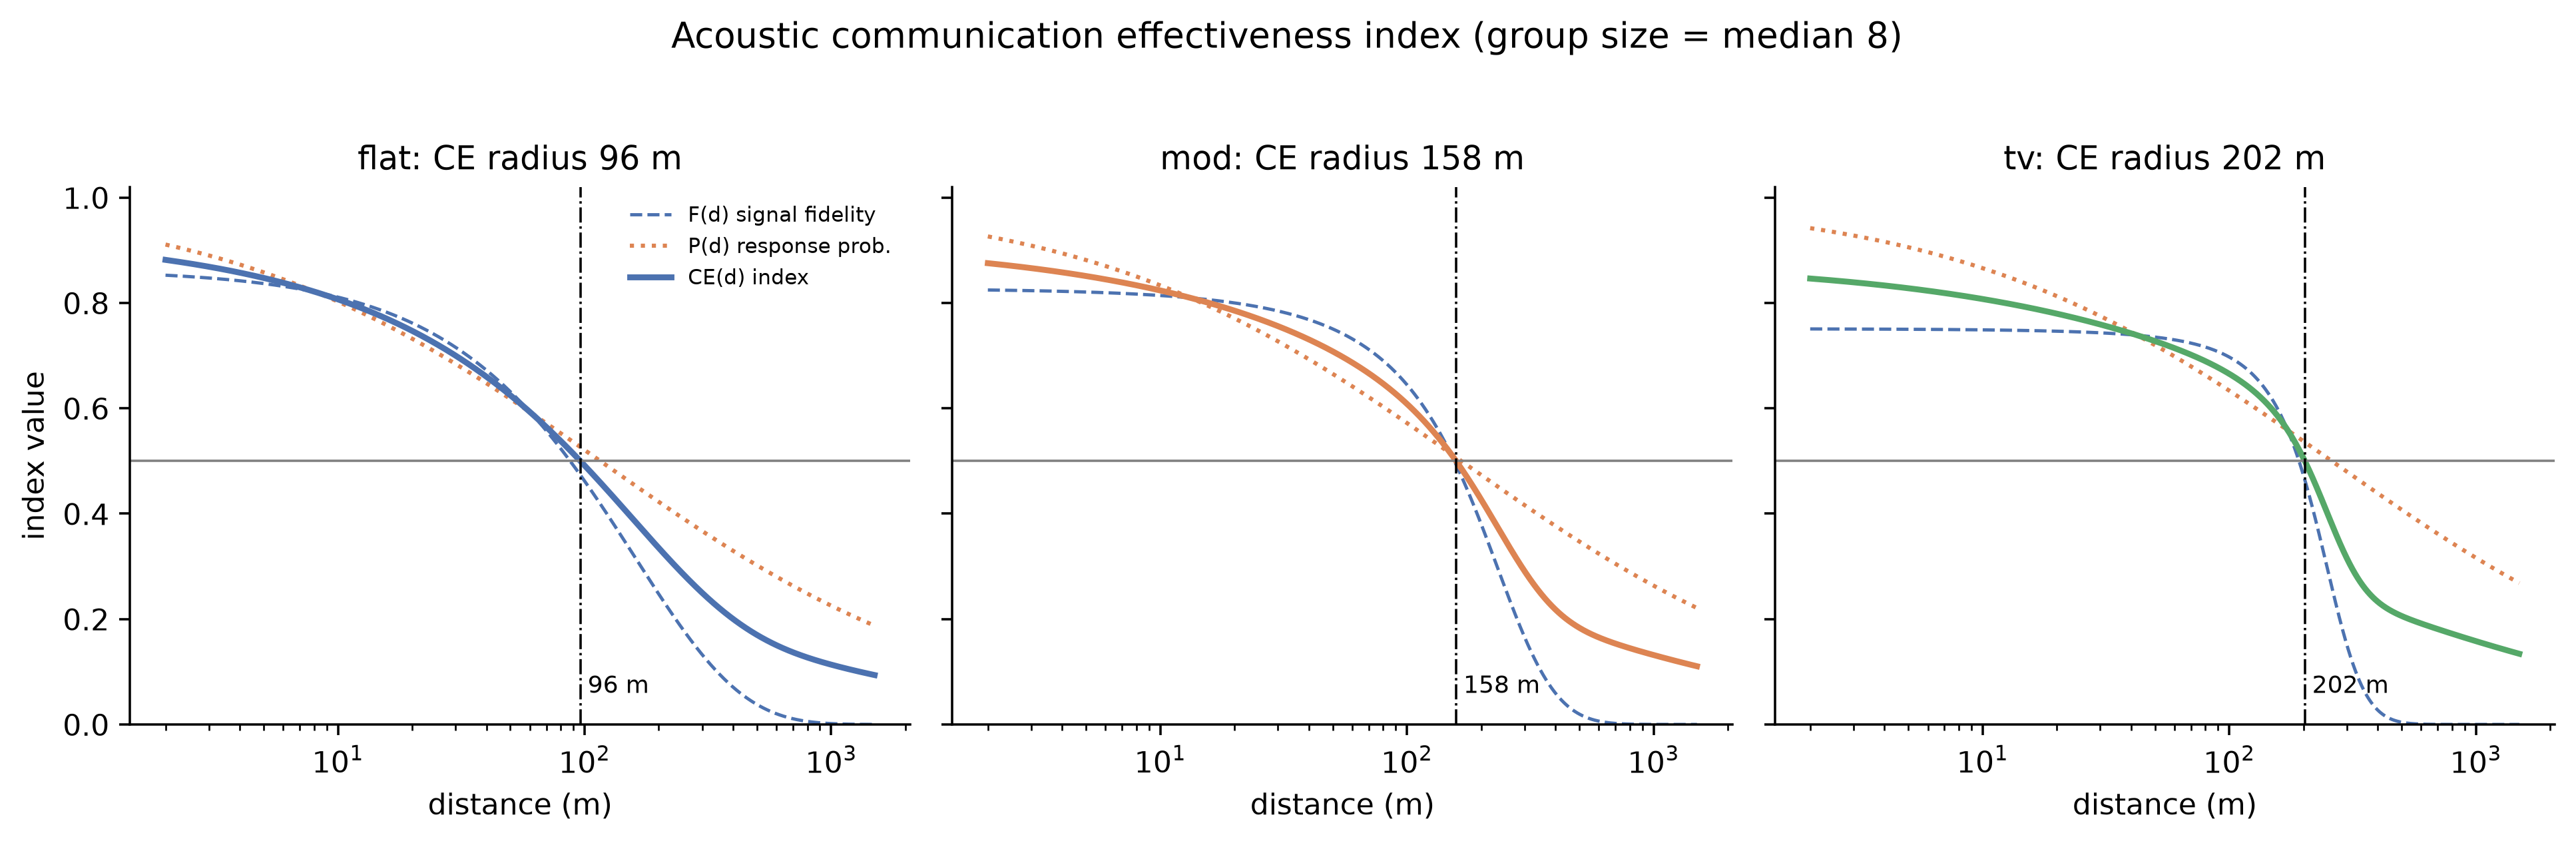
\includegraphics[width=\textwidth]{figures/fig10_ce_index.png}
\caption{Communication-effectiveness index (solid) and its two components (dashed: signal
fidelity; dotted: response probability) as a function of distance. The vertical
dash-dotted line marks the index radius at the $0.5$ threshold.}
\label{fig:ce}
\end{figure}

\subsection{Expected number of responders}

A second operational quantity is the expected number of penguins that respond to a single
playback. Because the response probability depends on group size, we average over the
empirical group-size distribution of the $278$ trials:
\begin{equation}
\mathbb{E}[R_c(d)]=\sum_{g} \pi(g)\, g\, P_c(d,g),
\end{equation}
where $\pi(g)$ is the observed relative frequency of group size $g$. This treats the
per-trial response probability as an individual response probability, which is a
simplification: the playback data record whether \emph{any} penguin in the group
responded, not how many, so the expected numbers inherit that assumption. At $50$ m the
expected numbers are $4.8$ (flat), $5.3$ (modulated) and $5.9$ (two-voice); at $200$ m
they are $3.0$, $3.5$ and $4.0$. The decline with distance is shallower than the decline
in response probability, because larger groups respond at a slightly lower per-trial rate
and the product partly offsets itself.

\begin{figure}[!ht]
\centering
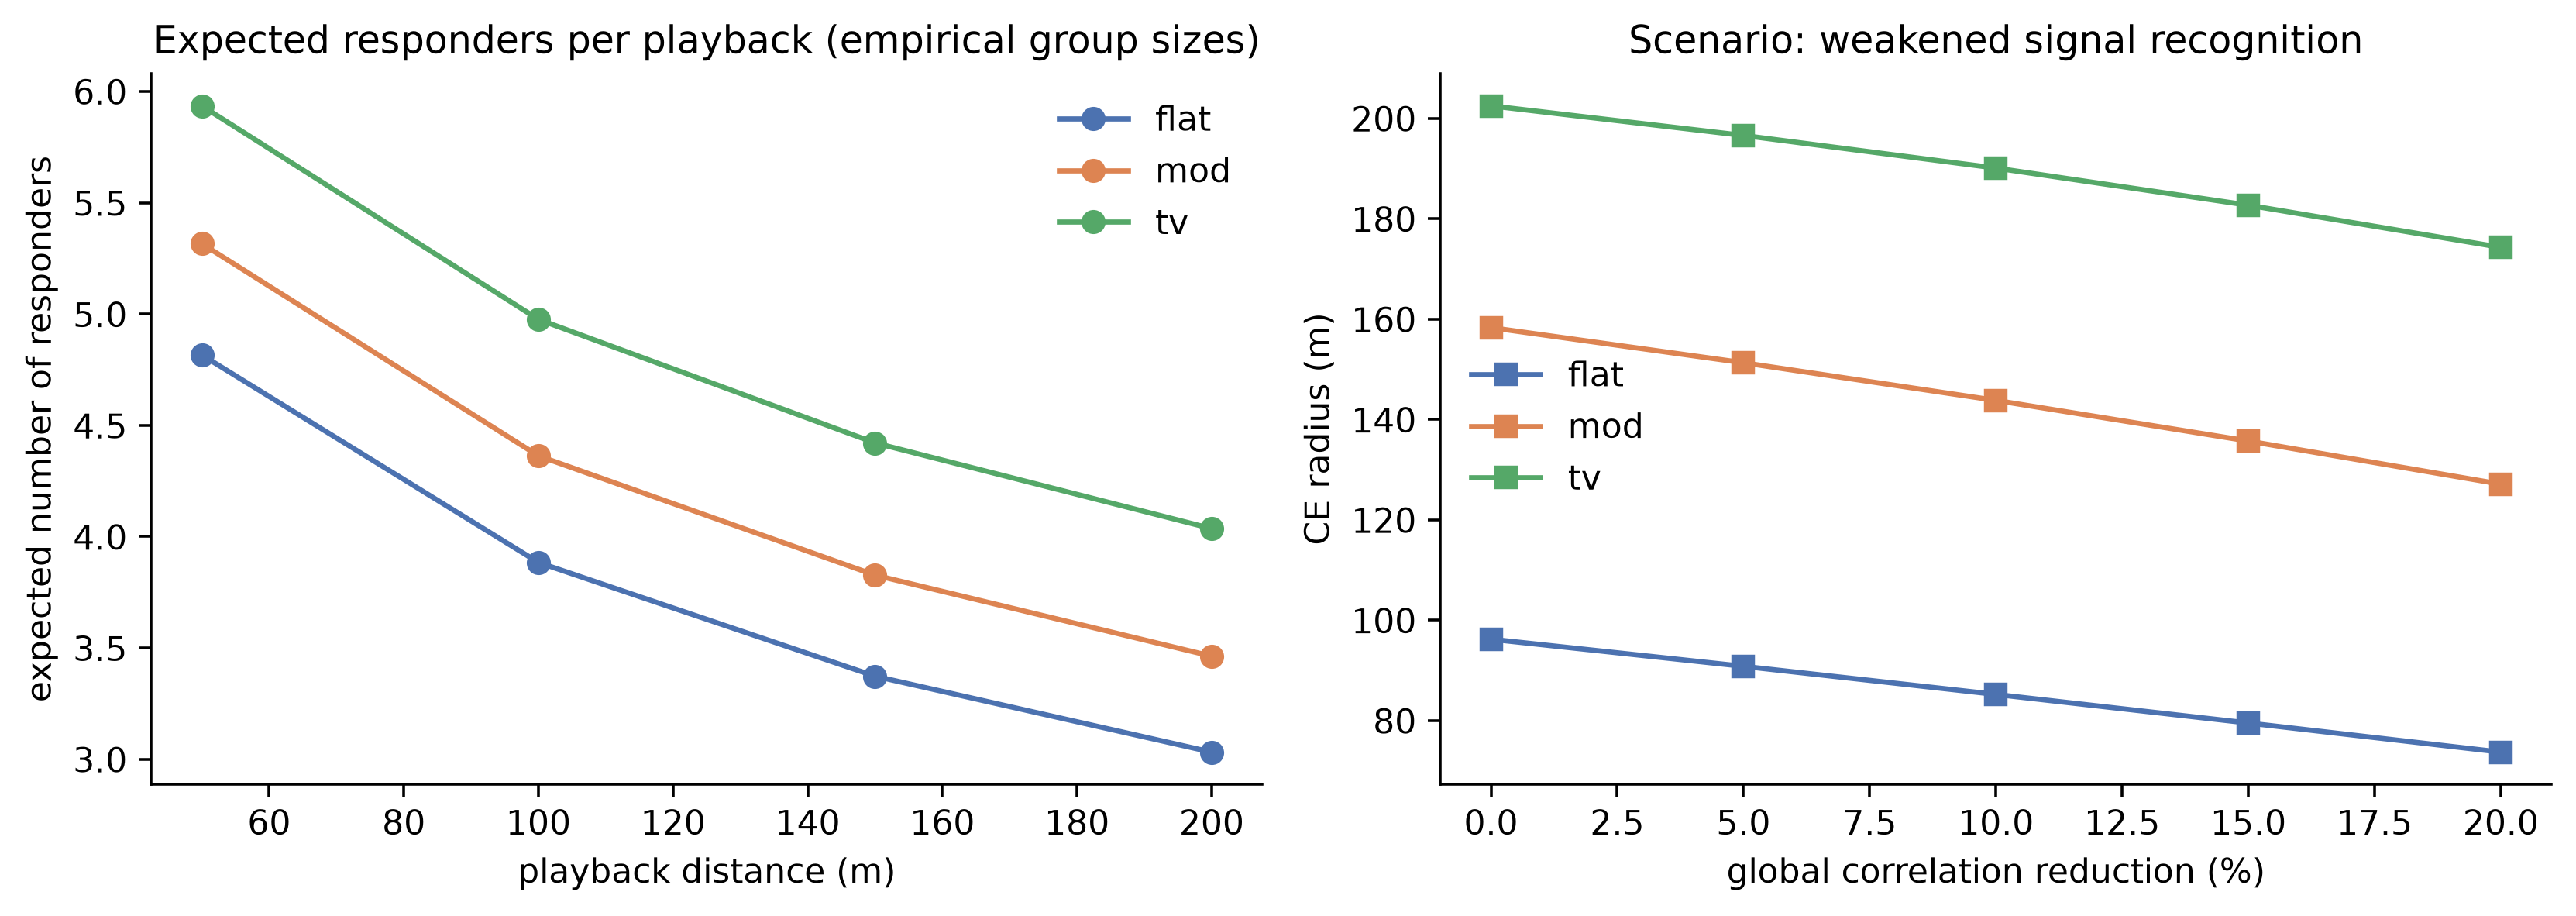
\includegraphics[width=\textwidth]{figures/fig11_scenarios.png}
\caption{Left: expected number of responders per playback as a function of distance.
Right: loss of effective range under a global reduction of signal correlation, the
scenario corresponding to increased ambient noise or adverse sea state.}
\label{fig:scen}
\end{figure}

\subsection{Scenarios: noise and weakened recognition}

Three stress tests were applied.

\paragraph{Raising the recognition threshold.} The recognition criterion is a statement
about the correlation between a degraded and the original signal, so it should be moved on
the fidelity curve $F_c(d)$, not the composite index. On $F_c(d)$ the ranges fall from $87$
to $58$ to $34$ m (flat), $156$ to $118$ to $76$ m (modulated) and $192$ to $157$ to $98$ m
(two-voice), matching Question~2. Applied instead as an index decision threshold on
$\mathrm{CE}_c(d)$---a distinct quantity that also encodes the response probability---the
same numbers give $96$ to $58$ to $30$ m, $158$ to $105$ to $54$ m and $203$ to $148$ to
$71$ m. Either way the ranking is preserved, but the loss is severe.

\paragraph{Global loss of signal correlation.} If environmental noise reduces every
correlation by $5\%$, $10\%$, $15\%$ or $20\%$, the flat-call radius falls from $96$ to
$91$, $85$, $80$ and $74$ m. Two-voice calls fall from $203$ to $197$, $190$, $183$ and
$174$ m. The response is close to linear and the ordering is again preserved, but the
absolute loss for the weakest call type is proportionally larger, so noise compresses the
differences between call types rather than reversing them.

\paragraph{Responder proportion.} If only a fraction of the observed group responds,
the expected number of responders scales by that fraction. At a quarter of the observed
rates, the expected numbers at $100$ m fall to $1.0$ (flat), $1.1$ (modulated) and $1.2$
(two-voice), which is the regime in which a single call no longer reliably recruits a
group.

\subsection{Implications and limitations}

Three conclusions follow. First, two-voice calls are the only call type that supports
communication beyond about $150$ m under a strict criterion, and they are therefore the
natural target for passive acoustic monitoring. Second, the binding constraint differs by
call type, which matters for management: protecting flat-call communication means
protecting the acoustic channel, whereas protecting two-voice communication is limited
more by masking of the received signal than by the animals' willingness to respond. Third,
the sensitivity to the signal-recognition threshold is larger than the sensitivity to a
global noise reduction of the same nominal magnitude, so management should be anchored to
a stated recognition criterion rather than to an unstated ``audible'' range.

The limitations are equally clear. The sample is small, the response models are
observational, and the playback data do not identify individual listeners, so the group
size effect may reflect either dilution of vigilance or repeated sampling of experienced
individuals. The propagation experiments were conducted at one site, and the decay curves
absorb any site-specific absorption into their parameters; transferring the radii to
another site would require a new calibration.

%=====================================================================
\section{Model evaluation}\label{sec:eval}

\paragraph{Internal validity.} Every classifier was evaluated by five-fold
cross-validation with a fixed seed, and every regression was checked against an
events-per-variable budget recorded before fitting. All reported radii are interior
solutions of the fitted curves.

\paragraph{Sensitivity.} For Question 2 the dominant uncertainties are sampling error
(about $\pm1$--$4$ m, from whole-recording bootstrap) and model form (about $20$ m for
flat calls, $50$ m for modulated calls and far more for two-voice calls). For Question 4
the index radius moves
by less than $6\%$ across a factor-of-two change in $w_1$, and by about $14$--$23\%$ under
a $20\%$ global loss of correlation.

\paragraph{Assumption checks.} Proportional hazards passes for head raising but fails for
the distance term in the vocalising model; proportional odds for the behaviour count is
rejected, and we switched to the multinomial model. Both failures are reported rather than
suppressed.

\paragraph{Threats to validity.} The absence of individual identification is the largest
threat, making the group-size coefficient ambiguous between a dilution effect and a
repeated-measures artefact. The censoring time is a surrogate for the unstated observation
window and is handled as a scenario assumption.

%=====================================================================
\section{Strengths and weaknesses}

\paragraph{Strengths.} The analysis is built around estimability rather than around model
sophistication. Three concrete decisions follow from this: the classifier is reported on a
feature set that excludes definitional variables and the leakage is quantified instead of
being hidden; every regression is fitted inside an events-per-variable budget, which is
why the approach behaviour is analysed with one covariate instead of diverging; and the
inverse problem that turns a threshold into a distance is reported with an explicit
reachability rule. The fidelity index is justified empirically by a principal component
analysis rather than by assertion, and the effective ranges are given as intervals that
separate sampling from model-form uncertainty.

\paragraph{Weaknesses.} The sample sizes are small, particularly for approaching, and the
acoustic classifier, even with engineered features, is only moderately accurate
($0.639$). The playback trials are pooled across contexts and sites without individual
identifiers, and the censoring time is inferred rather than observed. The
communication-effectiveness index uses equal weights, which we justify and test but which
remains a modelling choice.

%=====================================================================
\section{Conclusions}\label{sec:concl}

\begin{enumerate}[label=\textbf{(\arabic*)},leftmargin=*]
\item Of the six comparable acoustic measures, only peak frequency, the first fundamental
and the median frequency differ significantly, with small effect sizes
($\varepsilon^2\le0.10$). The apparent ease of separating the call types is an artefact of
definitional variables: a classifier using them reaches $0.944$, while acoustic shape alone
reaches $0.639$.

\item Acoustic fidelity falls from about $0.8$ at $4$ m to between $0.18$ and $0.28$ at
$256$ m. Effective ranges at the potential-recognition tier are $87$, $156$ and $192$ m
for flat, modulated and two-voice calls, with model-form bands of $[67,95]$,
$[138,206]$ and $[162,438]$ m. Two-voice calls are the most robust carrier at every
distance and every threshold.

\item Natural calls raise the response rate from $12.9\%$ to $64.8\%$; response
probability falls with distance and, weakly, with group size. Head raising responds
faster to natural calls (hazard ratio $4.9$) and vocalising responds much faster (hazard
ratio $21.7$). All $23$ approach events occurred in natural-call trials, so that effect
is a qualitative separation rather than an estimable odds ratio.

\item The communication-effectiveness index gives radii of $96$, $158$ and $203$ m for
flat, modulated and two-voice calls, falling to $34$, $76$ and $98$ m under a strict
$0.7$ recognition threshold; the ranking is stable under every scenario tested.

\item For conservation, the effective acoustic range of this species is on the order of
one to two hundred metres in typical coastal water, not kilometres, and it depends
strongly on the recognition criterion adopted; management that assumes a larger range is
optimistic.
\end{enumerate}

%=====================================================================
\section*{Recommendations for conservation practice}
\addcontentsline{toc}{section}{Recommendations for conservation practice}

\emph{Protect the near-field acoustic channel around foraging aggregations.} The weakest
call type carries less than $100$ m even at a permissive threshold, so broadband vessel
noise within a few hundred metres can mask communication for the whole group; a roughly
$200$ m exclusion radius around active aggregations is consistent with the two-voice
radius.

\emph{Treat passive acoustic monitoring as a short-range tool.} Monitoring that assumes
detection at kilometres will underestimate occupancy; with a potential-recognition range of
$87$--$192$ m, hydrophones should be spaced in hundreds of metres, not kilometres.

\emph{Prioritise masking reduction over source removal.} A $20\%$ global correlation loss
costs $14$--$23\%$ of range, whereas raising the recognition threshold from $0.5$ to
$0.7$ costs $49$--$62\%$; reducing impulsive noise during peak foraging is
therefore likely more effective than blanket noise limits.

These recommendations rest on a small observational sample from one region and are
order-of-magnitude guidance until replicated with marked birds.

%=====================================================================
\begin{thebibliography}{9}
\bibitem{kruskal} Kruskal W H, Wallis W A. Use of ranks in one-criterion variance
analysis[J]. Journal of the American Statistical Association, 1952, 47(260): 583-621.
\bibitem{dunn} Dunn O J. Multiple comparisons using rank sums[J]. Technometrics, 1964,
6(3): 241-252.
\bibitem{bh} Benjamini Y, Hochberg Y. Controlling the false discovery rate: a practical
and powerful approach to multiple testing[J]. Journal of the Royal Statistical Society:
Series B, 1995, 57(1): 289-300.
\bibitem{breiman} Breiman L. Random forests[J]. Machine Learning, 2001, 45(1): 5-32.
\bibitem{km} Kaplan E L, Meier P. Nonparametric estimation from incomplete
observations[J]. Journal of the American Statistical Association, 1958, 53(282): 457-481.
\bibitem{cox} Cox D R. Regression models and life-tables[J]. Journal of the Royal
Statistical Society: Series B, 1972, 34(2): 187-220.
\bibitem{burnham} Burnham K P, Anderson D R. Model Selection and Multimodel Inference: A
Practical Information-Theoretic Approach[M]. 2nd ed. New York: Springer, 2002, 60-80.
\bibitem{peduzzi} Peduzzi P, Concato J, Kemper E, et al. A simulation study of the number
of events per variable in logistic regression analysis[J]. Journal of Clinical
Epidemiology, 1996, 49(12): 1373-1379.
\bibitem{austin} Austin P C, Steyerberg E W. Events per variable (EPV) and the relative
performance of different strategies for estimating the out-of-sample validity of logistic
regression models[J]. Statistical Methods in Medical Research, 2017, 26(2): 796-808.
\end{thebibliography}

%=====================================================================
\newpage
\appendix
\section{Software and source code}

All analyses were run in Python 3.14.2 with pandas 2.3.3, NumPy 2.4.6, SciPy 1.18.1,
statsmodels 0.15.0, scikit-learn 1.9.1, lifelines 0.30.3 and scikit-posthocs 0.18.0.
Figures were produced with matplotlib 3.11.2 and seaborn 0.13.2. All random processes
use seed 42.

\begin{center}
\footnotesize
\begin{tabular}{ll}
\toprule
File & Purpose\\
\midrule
\texttt{00\_eda.py} & data audit, missingness and leakage checks\\
\texttt{01\_q1.py} & Question 1 statistics and classifiers\\
\texttt{02\_q2.py} & fidelity index, decay fits, ranges, bootstrap\\
\texttt{03\_q3.py} & Question 3 regressions and survival models\\
\texttt{04\_q4.py} & effectiveness index and scenario analysis\\
\texttt{05\_tables.py} & generates every table directly from the JSON results\\
\texttt{common.py} & shared paths, constants and plotting style\\
\bottomrule
\end{tabular}
\end{center}

\subsection{Stage 0: data audit}
\lstinputlisting[language=Python,basicstyle=\ttfamily\tiny]{code/00_eda.py}

\subsection{Question 1}
\lstinputlisting[language=Python,basicstyle=\ttfamily\tiny]{code/01_q1.py}

\subsection{Question 2}
\lstinputlisting[language=Python,basicstyle=\ttfamily\tiny]{code/02_q2.py}

\subsection{Question 3}
\lstinputlisting[language=Python,basicstyle=\ttfamily\tiny]{code/03_q3.py}

\subsection{Question 4}
\lstinputlisting[language=Python,basicstyle=\ttfamily\tiny]{code/04_q4.py}

\end{document}
